\documentclass[a4paper, twoside, 11pt]{article}
% It is needed to use this command for automatic compilation in VSCode
% !TEX program = lualatexmk

%DOCUMENT, PREAMBLE AND MACROS DESIGNED FOR LuaLaTeX%
\newcommand{\fbar}{\FloatBarrier}

\usepackage{amsmath} %matematic package%
\usepackage{amssymb} %for miscellaneous mathematical symbols, first usage was for tick symbol in math mode \checkmark%
\usepackage{textcomp} %for miscellaneous symbols%
%\usepackage{times} %times font%
\usepackage{graphicx} %enhanced support for craphics%
%\usepackage{mathptmx} %use Times as default text font, and provide maths support%
\usepackage{cmap} %mapování znaků - vyhledávání v pdf%
\usepackage[english]{babel}%CZ%
\usepackage[utf8]{inputenc}%kódování%
\usepackage[T1]{fontenc}%kódování%
\usepackage{multirow}%Multirow table support
\usepackage{float}%Improves the interface for defining floating objects such as figures and tables%
\usepackage{wasysym} %for various glyphs, symbols%

\usepackage{setspace}%spacing% 
\onehalfspacing

\usepackage{hyperref}
\hypersetup{
    colorlinks=true, %pokud nechci definovat citecolor=black aby byly odkazy citací černé, tak dám colorlinks=false,%
    bookmarks=true,
    linkcolor=black,
    citecolor=black,
    urlcolor=black,
}

%when using LuaLaTex, defining Times Fonts from your system - it has to be named like this and inserted ttf file in the folder of your tex file%
\usepackage{fontspec}
\selectlanguage{czech}
\setmainfont[Ligatures=TeX,BoldFont={Times New Roman Bold}] {Times New Roman}
                                
\setsansfont[Ligatures=TeX,BoldFont={* Bold}]{Times New Roman}
                                      
\setmonofont{CourierPrime-Regular}
 
%\usepackage[italic]{mathastext} %for text in math environment, better looking times then



%for CITATIONS URL to work, it is not needed when you are not using URL label%
\usepackage{url}
\usepackage{csquotes}
\usepackage[style=iso-numeric, backend=biber, isbn=true, urldate=iso,seconds=true, date=terse, datezeros=true, language=czech]{biblatex}
\addbibresource{src/bib/zdroje.bib} % BIB resources to import
%\DeclareUrlCommand\url{\def\UrlLeft{<}\def\UrlRight{>} \urlstyle{tt}}



%\usepackage{biblatex}
%END for citations%

%changing bibliography font%
\renewcommand*{\bibfont}{\fontspec{Times New Roman}}

\usepackage{comment} %For comments%
\usepackage{pdfpages}%for pdf pages%
\usepackage{enumerate}%For lists%
\usepackage{enumitem}%For Custom Numbering Nested Lists%
\setlist[enumerate]{label*=\arabic*.} %setting Number. numbering in lists%
\usepackage{tikz} %For vector graphics%
\usepackage{circuitikz}%For schemes%
\usepackage{pgf} %Post script graphics for tikz%

%pouze funguje v PDFLaTeX%
%\usepackage{tgtermes}%na times font, jiný nefunguje s vyhledáváním a copy%

%
\usepackage{placeins}%% for \FloatBarrier command that blocks floating with htbp! go over \FloatBarrier
\usepackage{mathrsfs}%packagee for math symbols for Laplace, Z transform etc., usage \mathscr{Z}
\usepackage{upgreek}%for upgreek symbols, specified tau \uptau
\usepackage{physics}% for derivations \dd
%this works only when using PDFLaTeX%
\usepackage[list=true,listformat=simple]{subcaption}
\usepackage[figurename=Fig.,font=small,labelfont=it,textfont=it]{caption} %for renaming figures instead of renewcommand, small for 11pt default is 10pt as needed in word template
\usepackage[tablename=Tab.,font=small,labelfont=it,
            textfont=it]{caption} %for renaming tables instead of renewcommand
            

% List of abbreviations and symbols
% Original code author: Jakub Kučera

\usepackage[nonumberlist,nopostdot,section=subsection,numberedsection]{glossaries}
% section = subsection is for glossaries title to appear as a subsection, numberedsection adds the subsec number

\newglossary[slg]{symbolslist}{symbol}{ntn1}{List of symbols}
\newglossary[slg]{abbreviationslist}{abbreviation}{ntn2}{List of abbreviations}

\makeglossaries

% include files with definitions
% PZ definitions
\newglossaryentry{abbreviation:soc}{
                type=abbreviationslist,
                name={SoC},
                description={System on a chip}
}

\newglossaryentry{abbreviation:ip}{
                type=abbreviationslist,
                name={IP},
                description={Intellectual property}
}
\newglossaryentry{abbreviation:fpga}{
                type=abbreviationslist,
                name={FPGA},
                description={Field Programmable Gate Array}
}
\newglossaryentry{abbreviation:nr}{
                type=abbreviationslist,
                name={NR},
                description={Newton Raphson}
}
\newglossaryentry{abbreviation:rtl}{
                type=abbreviationslist,
                name={RTL},
                description={Register Transfer Level}
}
\newglossaryentry{abbreviation:fsm}{
                type=abbreviationslist,
                name={FSM},
                description={Finite State Machine}
}
\newglossaryentry{abbreviation:cordic}{
                type=abbreviationslist,
                name={CORDIC},
                description={Coordinate Rotation Digital Computer}
}
\newglossaryentry{abbreviation:lut}{
                type=abbreviationslist,
                name={LUT},
                description={Look Up Table}
}
\newglossaryentry{abbreviation:cpu}{
                type=abbreviationslist,
                name={CPU},
                description={Central Processing Unit}
}
\newglossaryentry{abbreviation:isa}{
                type=abbreviationslist,
                name={ISA},
                description={Instruction Set Architecture}
}
\newglossaryentry{abbreviation:foss}{
                type=abbreviationslist,
                name={FOSS},
                description={Free and Open-Source Software}
}
\newglossaryentry{abbreviation:she}{
                type=abbreviationslist,
                name={SHE},
                description={Selective Harmonic Elimination}
}
\newglossaryentry{abbreviation:vsi}{
                type=abbreviationslist,
                name={VSI},
                description={Voltage Source Inverter}
}
\newglossaryentry{abbreviation:dc}{
                type=abbreviationslist,
                name={DC},
                description={Direct Current}
}
\newglossaryentry{abbreviation:vcd}{
                type=abbreviationslist,
                name={VCD},
                description={Value Change Dump}
}

\newglossaryentry{symbol:Pn}{
    type=symbolslist, % glossary
    name=$P_\text{n}$, % jméno v seznamu
    description={jmenovitý výkon stroje}, %popis
    symbol = (W),
    sort=P % seředit podle
}



\newglossarystyle{myStyleAbbreviations}{
\renewenvironment{theglossary}%
     {\begin{longtable}[l]{llp{\glsdescwidth}p{\glspagelistwidth}}}%
     {\end{longtable}}%
  \renewcommand*{\glossaryheader}{}%
  \renewcommand*{\glsgroupheading}[1]{}%
  \renewcommand{\glossentry}[2]{%
  \glsentryitem{##1} \glstarget{##1}{##2} &
    \textbf{\glossentryname{##1}} &
    \glossentrydesc{##1} &
    ##2\tabularnewline
  }%
  \renewcommand*{\glsgroupskip}{}%  Pokud chci seskupovat podle abeced: \renewcommand*{\glsgroupskip}{ & \\}
}


\newglossarystyle{myStyleSymbols}{
  \renewenvironment{theglossary}%
    {\begin{longtable}[l]{llp{\glsdescwidth}p{\glspagelistwidth}}}%
    {\end{longtable}}%
  \renewcommand*{\glossaryheader}{}%
  \renewcommand*{\glsgroupheading}[1]{}%
  \renewcommand{\glossentry}[2]{%
    \glsentryitem{##1} \glstarget{##1}{\glossentryname{##1}} &
    \glossentrysymbol{##1} &
    \glossentrydesc{##1} &
    ##2\tabularnewline
  }%
  \renewcommand{\subglossentry}[3]{%
     &
     \glssubentryitem{##2}%
     \glossentrysymbol{##2} &
     \glstarget{##2}{\strut}\glossentrydesc{##2} & ##3\tabularnewline
  }%
  \renewcommand*{\glsgroupskip}{%
   }% Pokud chci seskupovat podel abecedy  \ifglsnogroupskip\else & & &\tabularnewline\fi
}
\renewcommand{\glossarypreamble}{\vspace*{-\baselineskip}} % deleting line after glossaries title

            %this works with LuaLaTex and fontspec package%
 \DeclareCaptionFont{times}{\fontspec{Times New Roman Italic}}

%labelfont and textfont defined here only works with previous declarecaptionfont times and fontspec%
\captionsetup{labelfont=times, textfont=times, labelsep=space}%no separator in captions
%

%\bibliographystyle{czechiso} %czechiso.bst in folder is needed for this style to work, available at http://www.fit.vutbr.cz/~martinek/latex/czechiso.html%

%\hyperref[label]{text}% Help for targeting labels

\usepackage{chngcntr} %for numbered figures with sections
\usepackage{tocloft}%better TOC

%\usepackage{a4wide}%širší a4%
\usepackage[inner=3cm,outer=2cm,top=2.5cm,bottom=2.5cm,footskip=1cm]{geometry}%for propper margins
\usepackage{textcase}%for making text uppercase without caps \MakeTextUppercase
 
 
\usepackage{titlesec}%for spacing text after sections
\usepackage{parskip}[]%for working \parskip
\newcommand{\sectionbreak}{\clearpage}%maybe for SECTIONS on a new page

\usepackage[titletoc]{appendix}%For appendix - přílohy, titletoc is crucial
%\renewcommand{\appendixname}{Příloha}

\setlength{\parindent}{0.5cm}%setting indent of paragraph to 0.5cm
\setlength{\parskip}{0em}%setting parskip to 0 for \titleformat to work properly with parskip package

\usepackage{colortbl}%for colored cells
\usepackage{xcolor}%for colors
\definecolor{ctublue}{HTML}{0065BD}%defining ctu color
\definecolor{ctugreen}{HTML}{A2AD00}
\definecolor{ctured}{HTML}{C60C30}
\definecolor{ctuyellow}{HTML}{F0AB00}
\definecolor{ctugreenyblue}{HTML}{00B2A9}
\definecolor{ctulightblue}{HTML}{6AADE4}
\definecolor{ctuorange}{HTML}{E05206}
\definecolor{lightgray}{HTML}{D1D5DB}
\definecolor{codeblue}{HTML}{D9E2F3}


\titlespacing*{\section}{0em}{1em}{-\parskip}%spacing text after sections from titlesec package
\titlespacing*{\subsection}{0em}{1em}{-\parskip}%spacing text after sections from titlesec package
\titlespacing*{\subsubsection}{0em}{1em}{-\parskip}%spacing text after sections from titlesec package

%when you want sectin/sub/subsub to be black, delete \color{ctublue}
\titleformat{\section}{\color{ctublue}\fontspec{Times New Roman}\fontsize{15}{15}\bfseries}{\thesection}{2.1em}{}%defining title sizes by word template
\titleformat{\subsection}{\color{ctublue}\fontspec{Times New Roman}\fontsize{14}{14}\bfseries}{\thesubsection}{1.53em}{}%defining title sizes by word template
\titleformat{\subsubsection}{\color{ctublue}\fontspec{Times New Roman}\fontsize{13}{13}\bfseries}{\thesubsubsection}{1em}{}%defining title sizes by word template


\usepackage{ctable}%imports xtable with booktabs
\usepackage{multicol}

\usepackage{listings}%for code environments - \begin{lstlisting}


\definecolor{codegreen}{rgb}{0,0.6,0}
\definecolor{codegray}{rgb}{0.5,0.5,0.5}
\definecolor{codepurple}{rgb}{0.58,0,0.82}
\definecolor{backcolour}{rgb}{0.95,0.95,0.92}


% solving problems with ) literal to be coded in lstlisting as it should be
\makeatletter
\patchcmd{\lsthk@SelectCharTable}{)}{`}{}{} 
\makeatother 

\lstdefinestyle{zakopal}{
    backgroundcolor=\color{codeblue},   
    commentstyle=\color{codegray},
    keywordstyle=\color{ctured},
    numberstyle=\tiny\color{codegray},
    stringstyle=\color{ctuorange},
    basicstyle=\ttfamily\small,
    breakatwhitespace=false,         
    breaklines=true,                 
    captionpos=b,                    
    keepspaces=true,                 
    numbers=left,                    
    numbersep=5pt,                  
    showspaces=false,                
    showstringspaces=false,
    showtabs=false,                  
    tabsize=2
}
\lstset{style=zakopal}
\renewcommand{\lstlistingname}{Code}% renaming Listing -> Kód 
\renewcommand{\lstlistlistingname}{List of codes}% renaming List of Listings -> Seznam kódů

\lstdefinelanguage{SCL}
{morekeywords={FUNCTION_BLOCK,BEGIN,NOT,END_FUNCTION_BLOCK,FUNCTION,VOID,VAR_INPUT,END_VAR,VAR_IN_OUT,IF,
THEN,END_IF,END_FUNCTION,BOOL,FALSE,TRUE},
sensitive=false,
morecomment=[l]{//},
morestring=[b]",
literate={;}{{\textcolor{ctuorange}{;}}}{1}
{:}{{\textcolor{ctuorange}{:}}}{1}
{)}{{\textcolor{ctuorange}{)}}}{1}
{(}{{\textcolor{ctuorange}{(}}}{1}
{=}{{\textcolor{ctuorange}{=}}}{1}
{,}{{\textcolor{ctuorange}{,}}}{1},} %basic SCL language for siemens defined%

\lstdefinelanguage{xdc}
{morekeywords={set_property, current_design, get_ports},
sensitive=false,
morecomment=[l]{\#}} %basic xdc file in Vivado syntax highlighting%

\lstdefinelanguage{xsct}
{morekeywords={xsct, hsi, open_hw_design, -createdts, -hw, -zocl, -platform-name, -overlay, -compile, -out, exit, -git-branch},
alsoletter={-},
sensitive=false,
morecomment=[l]{\#}} %xsct (Xilinx Software Command-Line Tools)%


\lstdefinelanguage{Text}
{morekeywords={},
alsoletter={-},
sensitive=false,
morecomment=[l]{//},
morecomment=[l]{\#}} %basic text%

\lstdefinelanguage{devicetree}
{morekeywords={chosen, bootargs, stdout-path, compatible, status},
alsoletter={-},
stringstyle=\color{ctuorange},
moredelim=[s][\color{ctuorange}]{"}{"},
sensitive=false,
morecomment=[l]{\#},
literate={\{}{{\textcolor{ctured}{\{}}}{1}
{\}}{{\textcolor{ctured}{\}}}}{1}
} %devicetree%

\lstdefinelanguage{json}
{morekeywords={},
upquote=true,
morestring=[b]",
stringstyle=\color{ctuorange},
moredelim=[s][\color{ctuorange}]{"}{"},
sensitive=false,
morecomment=[l]{\#},
literate=
     *{0}{{{\color{ctured}0}}}{1}
      {1}{{{\color{ctured}1}}}{1}
      {2}{{{\color{ctured}2}}}{1}
      {3}{{{\color{ctured}3}}}{1}
      {4}{{{\color{ctured}4}}}{1}
      {5}{{{\color{ctured}5}}}{1}
      {6}{{{\color{ctured}6}}}{1}
      {7}{{{\color{ctured}7}}}{1}
      {8}{{{\color{ctured}8}}}{1}
      {9}{{{\color{ctured}9}}}{1}
      {\{}{{{\color{ctured}{\{}}}}{1}
      {\}}{{{\color{ctured}{\}}}}}{1}
      {[}{{{\color{ctured}{[}}}}{1}
      {]}{{{\color{ctured}{]}}}}{1},
} %json%

\lstdefinelanguage{pseudocode}
{morekeywords={if, else, positive, negative, edge, end},
alsoletter={-},
stringstyle=\color{ctuorange},
moredelim=[s][\color{ctuorange}]{"}{"},
sensitive=false,
morecomment=[l]{\//},
literate={\{}{{\textcolor{ctured}{\{}}}{1}
{\}}{{\textcolor{ctured}{\}}}}{1}
{(}{{{\color{ctured}{(}}}}{1}
{)}{{{\color{ctured}{)}}}}{1}
{\&}{{{\color{ctublue}{\&}}}}{1}
{=}{{{\color{ctublue}{=}}}}{1}
{<}{{{\color{ctublue}{<}}}}{1}
{>}{{{\color{ctublue}{>}}}}{1}
} 
%%change in previous commands 2.1 em , 1.53em and 1em to 1em to be easy indented not the same
\begin{document}
\fontspec{Times New Roman}

\counterwithin{figure}{section}%changing counter of figure, at each section the numbering resets
\counterwithin{table}{section}%changing counter of table, at each section the numbering resets
\counterwithin{equation}{section}%changing counter of equation, at each section the numbering resets

\counterwithin{lstlisting}{section}%counter of lstlist - codes, reseting at each section%


\renewcommand{\thefigure}{\thesection~-~\arabic{figure}}%defining style of countering
\renewcommand{\thetable}{\thesection~-~\arabic{table}}
\renewcommand{\theequation}{\thesection~-~\arabic{equation}}
\renewcommand{\thelstlisting}{\thesection~-~\arabic{lstlisting}}%delfining style for lstlisting codes, needs to be after begin document as previous renewcommand%

\renewcommand*{\cftsecdotsep}{1}  % use dots in the section entries and their step
\renewcommand*{\cftsubsecdotsep}{1}
\renewcommand*{\cftsubsubsecdotsep}{1}
\renewcommand*{\cftsecnumwidth}{4em} % increase space for Roman numerals
\renewcommand*{\cftsubsecnumwidth}{4em} %numbering width
\renewcommand*{\cftsubsubsecnumwidth}{4em} %numbering width
\renewcommand*{\cftsubsubsecindent}{0em}%no indent for subsubsection
\renewcommand*{\cftsubsecindent}{0em}%no indent for subsection
\renewcommand*{\cftsecindent}{0em}%no indent for subsection



\renewcommand*{\cftfigdotsep}{1}  % use dots in the figure entries and their step
\renewcommand*{\cftfignumwidth}{4em}
\renewcommand*{\cftfigindent}{0em}

\renewcommand*{\cfttabdotsep}{1}  % use dots in the figure entries and their step
\renewcommand*{\cfttabnumwidth}{4em}
\renewcommand*{\cfttabindent}{0em}

\renewcommand{\cftsecfont}{\fontspec{Times New Roman}\large \bfseries}
\renewcommand{\cftsubsecfont}{\fontspec{Times New Roman}}
\renewcommand{\cftsubsubsecfont}{\fontspec{Times New Roman}}

\renewcommand{\cftfigfont}{\fontspec{Times New Roman}}
\renewcommand{\cfttabfont}{\fontspec{Times New Roman}}

\renewcommand*\contentsname{\textcolor{ctublue}{\MakeTextUppercase{\fontspec{Times New Roman}Table of Contents}}}
\renewcommand{\listtablename}{{\fontspec{Times New Roman}\textcolor{ctublue}{\MakeTextUppercase{{List of tables}}}}}
\renewcommand{\listfigurename}{{\fontspec{Times New Roman}\textcolor{ctublue}{\MakeTextUppercase{{List of figures}}}}}



%\renewcommand{\thefigure}{\arabic{section}.\arabic{figure}}%changing figure name to be section.subsection. but do no reset
\setcounter{figure}{0}

\begin{titlepage}
	\begin{center}

\begin{figure}[H]
	\begin{center}
		
\includegraphics[scale=1]{src/misc/symbol_cvut_konturova_verze.pdf}
	\end{center}
\end{figure}
	{\Large{\textbf{CZECH TECHNICAL UNIVERSITY IN PRAGUE}}}\\
	{\textbf{Faculty of Electrical Engineering}}\\
	{\textbf{Department of Electric Drives and Traction}}
	
	\vspace{3cm}
	
	
	{\Large\textbf{Name of the report}}
	
	\vspace{1cm}
	
	%{\Large\textbf{Possibilities of Using SoC Platform Processors for Controlling Electric Drives}}
	
	%\vspace{2cm}
	
	Technical report\\
	
	\end{center}
	
	\vspace{3cm}
	
	%\noindent Studijní program: Elektrotechnika, Energetika a Management\\
	%\noindent Studijní obor: Elektrické pohony
	
	\vspace{0.5cm}
	%\noindent Vedoucí práce: doc. Ing. Jan Bauer, Ph.D.
	
	\vfill
	
\begin{center}

	\large{\textbf{Petr Zakopal}}\\
	\large{\textbf{Prague 2023}}
	\end{center}
\end{titlepage}


\newpage
%\pagenumbering{arabic} to arabic page numbering
\pagenumbering{gobble} %disabling page numbering

\newpage


%%ZADÁNÍ PRÁCE
%verze pro TISK - jen s NEW PAGE


%ONLINE VERZE - se zadáním BEZ PODPISŮ
% online verze - odkomentovat následující dva řádky
%\null\newpage
%\includepdf[]{src/docs/zadani_bez_podpisu.pdf}

%\newpage
%\cleardoublepage
\null\newpage

\pagenumbering{Roman}
\setcounter{page}{2}%%3 NUTNO řešit dle zadání etc.

% \noindent \textcolor{ctublue}{{\Large{\textbf{\MakeTextUppercase{Prohlášení}}}}}\\
% 			Prohlašuji, že jsem předloženou práci vypracoval samostatně a že jsem uvedl veškeré použité informační zdroje v~souladu s~Metodickým pokynem o~dodržování etických principů při přípravě vysokoškolských závěrečných prací.\\
% 		\vspace{1.5cm}
		
	

% 	\noindent	V~Praze dne \rule{3.5cm}{0.4pt} \hspace{6.6cm}  \rule{4cm}{0.4pt}
	
% 	\hspace{12.65cm}Petr Zakopal


% 		\vspace{14cm}
		
% 	\noindent	\textcolor{ctublue}{{\Large{\textbf{\MakeTextUppercase{Poděkování}}}}}\\
% 	Tímto bych rád poděkoval vedoucímu této práce doc. Ing. Janu Bauerovi, Ph.D. za skvělé vedení práce a cenné rady při jejím vytváření. Dále bych rád poděkoval všem, kteří mě v~mém dosavadním studiu podporovali.
		


%%ABSTRAKT%%

% \newpage
% %\addcontentsline{toc}{section}{3\quad Abstrakt a klíčová slova}%Added citations to TOC%
% %\begin{comment}
% \begin{minipage}[t]{7.37cm}
% 		%\raggedright
% 	\textcolor{ctublue}{\Large{\textbf{\MakeTextUppercase{Abstrakt}}}}\\
	
% \end{minipage}%
% \hfill% --- important, otherwise it wont be so nice
% \begin{minipage}[t]{7.37cm}
% 		\textcolor{ctublue}{\Large{\textbf{\MakeTextUppercase{Abstract}}}}\\
		
% \end{minipage}
% %\end{comment}
% 	%\textcolor{ctublue}{\Large{\textbf{\MakeTextUppercase{Abstrakt}}}}\\

% 	%\textcolor{ctublue}{\Large{\textbf{\MakeTextUppercase{Abstract}}}}\\

% \newpage
\tableofcontents
\newpage%
\flushbottom %vyčištění stránky
\newpage
\vspace{0pt}
\listoffigures %seznam obrázků
\flushbottom %vyčištění stránky
\newpage
\listoftables
\flushbottom
\newpage


\pagenumbering{arabic} %to arabic page numbering - enabling page numbering after gobble which disabled page numbering
\pagenumbering{gobble}
\null\newpage
% \null\newpage %PŘI VERZI ONLINE
\setcounter{page}{1}
\pagenumbering{arabic}
\fontspec{Times New Roman}

\section{Introduction}
This is the introduction.

\flushbottom %vyčištění stránky
\newpage
%konec úvodu

\section{Calculating the division of fixed point numbers}\label{sec:calculating-the-division-of-fixed-point-numbers}
Usually, when using numerical methods to solve the transcendetal equations, there is a need to calculate the division of two input numbers. Even for solving one set of two equations with Newton Raphson (\gls{abbreviation:nr}) method, the calculation of reciprocal value of the Jacobian determinant is needed.\par
There are available some \gls{abbreviation:ip} blocks, which are capable of calculating the division of two numbers, but the blocks are usually vendor specific intellectual property \gls{abbreviation:ip} \cite{amd-xilinx-vivado-divider-ip-block} or feature low performance \cite{burke-fixed-point-math-library}.\par
The negative side of vendor specific \gls{abbreviation:ip} is, that it is hard to use them with any other \gls{abbreviation:fpga} chip than the vendor specific. On the other hand the vendor specific \gls{abbreviation:ip} is usually optimized to use the specific type of resources available at the vendor's chip whci resolves in better performance.\par
To preserve the compatibility of the design with multiple vendors, the custom solution for division design based on the very known Newton Rapshon (\gls{abbreviation:nr}) algorithm was developed. \cite{burke-fixed-point-math-library}

\subsection{Newton Rapshon algorithm for calculating the division}\label{subsection:newton-raphson-algorithm-for-calculating-the-division}
General Newton Raphson (\gls{abbreviation:nr}) algorithm is a well known way how to solve equations the numerical way. It is the reason why it is utilized in many algorithms. However, the negative aspect of \gls{abbreviation:nr} is that it's convergency strongly depends on initial values of unknown variables. When the initial variables are chosen poorly, the performed number of iterations before the convergency is reached can be high.\par
To reach the fastest convergency possible (determined in number of iterations) apart from the scaling the dominator into the interval [0.5,1] the initial value calculation formula should be utilized. \cite{burke-fixed-point-math-library}
The initial value formula \ref{eq:initial-nr-value-formula} is applied after the scaling of denominator is performed. The algorithm developed for the appropriate scaling is explained in the \hyperref[subsec:calculating-number-of-bits-to-shift-the-denominator]{\textit{Calculating number of bits to shift the denominator}}.

\begin{equation}\label{eq:initial-nr-value-formula}
x_0 = \frac{48}{17} - \frac{32}{17} D,
\end{equation}
where the $x_0$ is the initial value for \gls{abbreviation:nr} algorithm and $D$ is the denominator value for calculating the expression $N/D$.\par
Because of the fixed point number format \textit{Q32.15} is used, the fractional numbers in equation \ref{eq:initial-nr-value-formula} are rounded to 2.8229 (32'b00000000000000010\_110100101011000 in binary)\newline and 1.8819 (32'b00000000000000001\_111000011100101 in binary) respectively.\par
After the initial value $x_0$ is calculated, the \gls{abbreviation:nr} algorithm is performed. The idea for using \gls{abbreviation:nr} algorithm to calculate the division of $N/D$ is to trade the division for a multiplication, which can be synthetized in the \gls{abbreviation:fpga} fabric. For the \gls{abbreviation:nr} algorithm the function which root is $1/D$ is crucial. There may be many functions, which root is the searched value $1/D$ but the most trivial is eq. \ref{eq:equation-with-appropriate-root}.\par

\begin{equation}\label{eq:equation-with-appropriate-root}
  \text{F} (x) = \frac{1}{x} - D.
\end{equation}

For the derivative at the point of $x_i$ then applies eq. \ref{eq:nr-division-derivative-at-the-point}.

\begin{equation}\label{eq:nr-division-derivative-at-the-point}
  \frac{\dd F(x_i)}{\dd x} = F'(x_i) = \frac{F (x_{i+1}) - F (x_i)}{x_{i+1}-x_i}.
\end{equation}

Because finding root of the equation \ref{eq:equation-with-appropriate-root}, the value of $F (x_{i+1})$ is set to be zero. After separating the $x_{i+1}$ value of the eq. \ref{eq:nr-division-derivative-at-the-point} and derivating the function $F (x_i)$ the obtained algorithm for a value $x_{i+1}$ is obtained in eq. \ref{eq:derivative-nr-new-value-algorithm}.\par

\begin{equation}\label{eq:derivative-nr-new-value-algorithm}
  x_{i+1} = -\frac{F (x_i)}{F' (x_i)} + x_i = - \frac{F (x_i)}{-\frac{1}{x_i^2}} + x_i = (\frac{1}{x_i} - D) x_i^2 + x_i = x_i - D x_i^2 + x_i = 2 x_i - D x_i^2.
\end{equation}

Usually, the iterative algorithm is stopped, when the value $F(x_{i+1}) - F(x_i)$ (called defect) reaches certain value set by the stop condition. However, in this algorithm, the stop condition is not yet implemented. Based on the observation carried on the N-R algorithm the obtained result is sufficient after 5 iterations.

The mathematically expressed algorithm is then transformed into calculation flow suitable for implementing in the FPGA. The top module design for this algorithm is presented in the section \hyperref[subsubsec:division-top-module-design]{\textit{Top module design}}, the control and data unit for calculating the value $x_{i+1}$ is presented in the \hyperref[subsubsec:division-allocation-and-timing]{\textit{Allocation and Timing}}

\subsection{IP block design}\label{subsec:division-ip-block-design}
The design of this division unit is separated into 4 main modules:
\begin{itemize}
  \item the \textbf{data unit module}, used for manipulating data and making calculation operations,
  \item the \textbf{control unit module}, used for controlling the \textbf{data unit module} and \textbf{scaling unit module}, this unit is a Finite State Machine (\gls{abbreviation:fsm}),
  \item \textbf{scaling unit module}, used for calculating the number of bits needed for shifting the denominator value to the interval [0.5,1].
\end{itemize}
\subsubsection{Top module design}\label{subsubsec:division-top-module-design}
The top module wraps all of the presented modules (\textbf{data unit module}, \textbf{control unit module}, \textbf{scaling unit module}). The basic structure of connected modules in this top design is depicted in the fig. \ref{fig:division-top-module}. Thanks to this wrapper it is possible to test the created modules with Verilog Testbench, Verilator \cite{verilator} or Cocotb \cite{cocotb}.
\begin{figure}[htbp!]
  \centering
  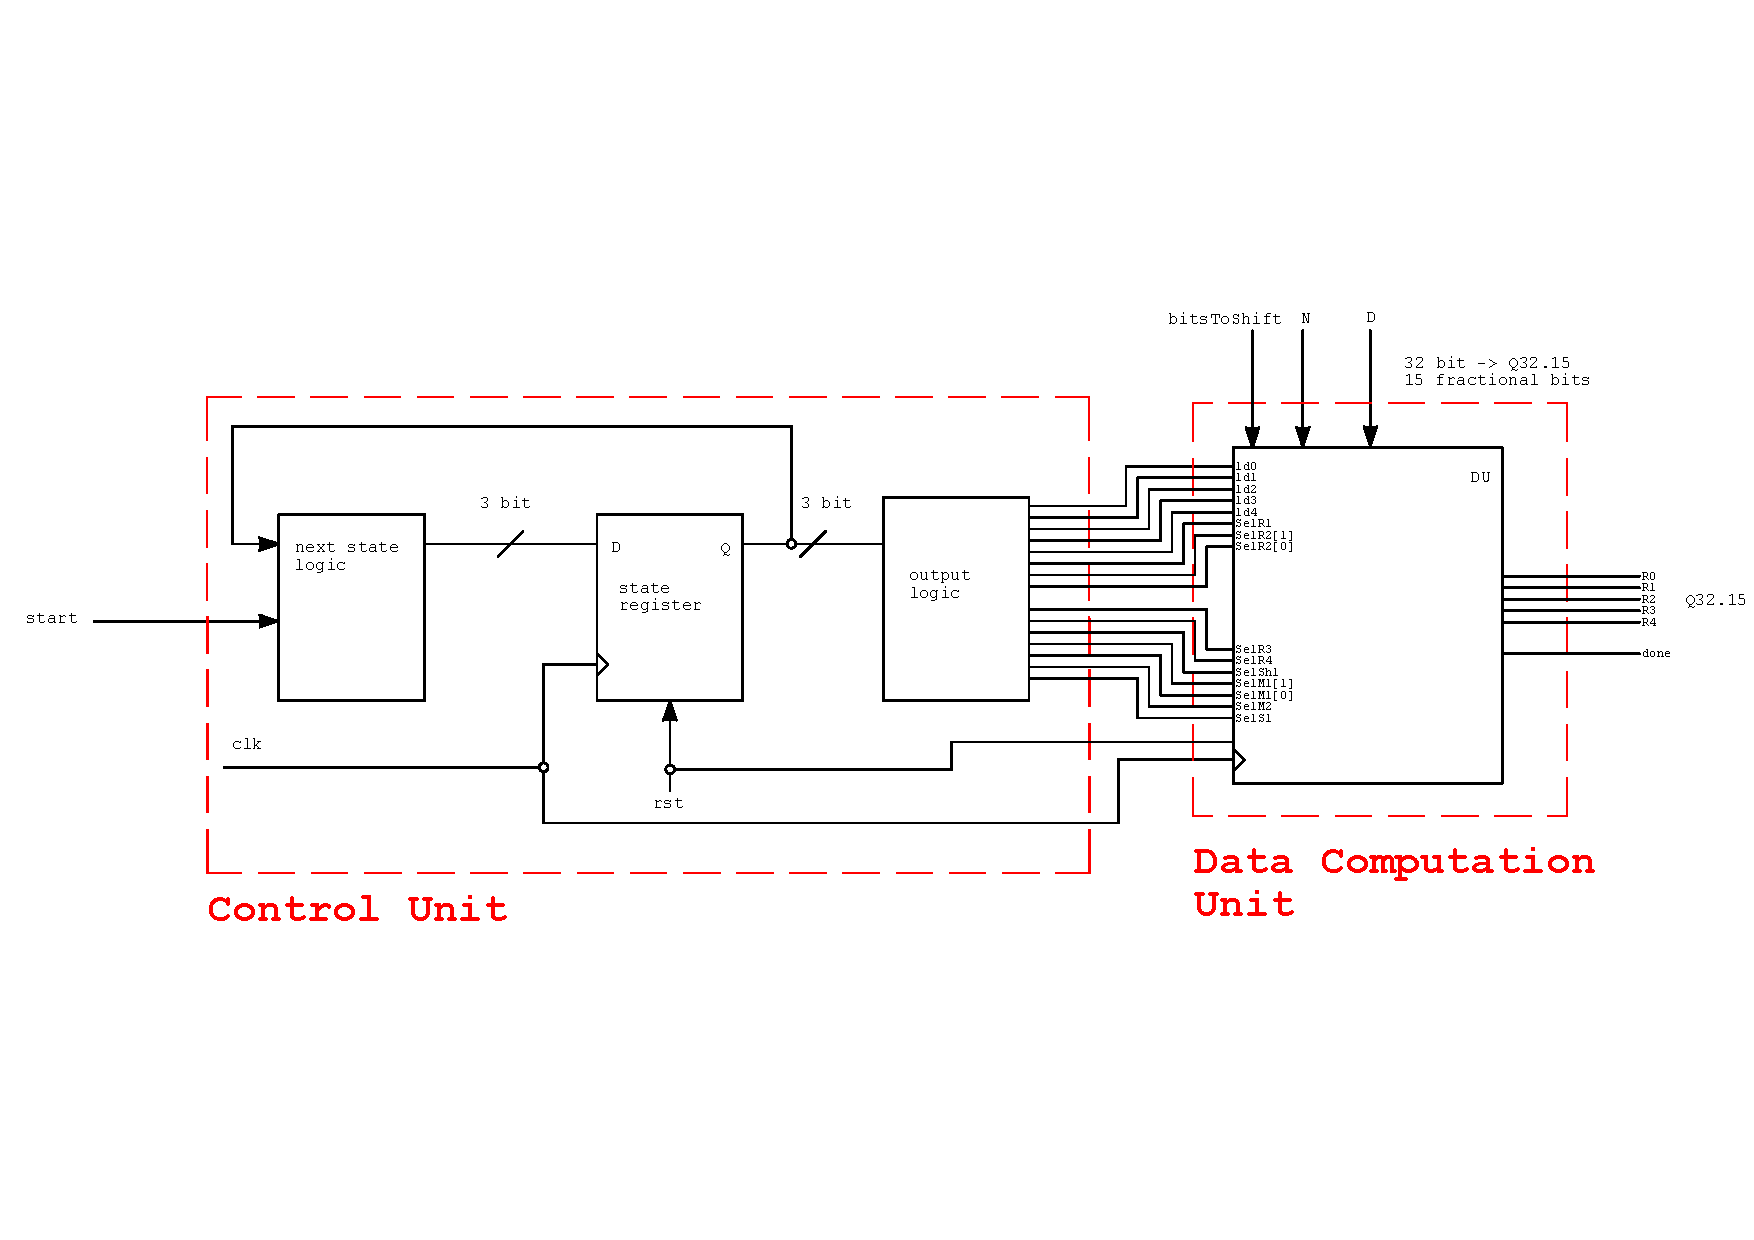
\includegraphics[width=1\textwidth]{src/pdf/top-module.pdf}
   \caption{Top module design for the \gls{abbreviation:ip} block design.}
  \label{fig:division-top-module}
\end{figure}



\fbar
\subsubsection{Allocation and Timing}\label{subsubsec:division-allocation-and-timing}
The diagram which describes the data flow and timing by steps of the algorithm is displayed in the figure \ref{fig:division-allocation-timing}.\par
The whole algorithm consists of nine steps. The first four steps are used for calculating the initial value of $x_0$ as described in the equation \ref{eq:initial-nr-value-formula}. The steps \textit{S4} to \textit{S8} are for calculating the next search value of $x_{i+1}$, the root of the equation \ref{eq:equation-with-appropriate-root} so the searched value of $1/D$. The next iteration starts at the step labeled as \textit{S5}. The iterative process continues till the stop condition (eg. number of iterations) is met.
\begin{figure}
  \centering
  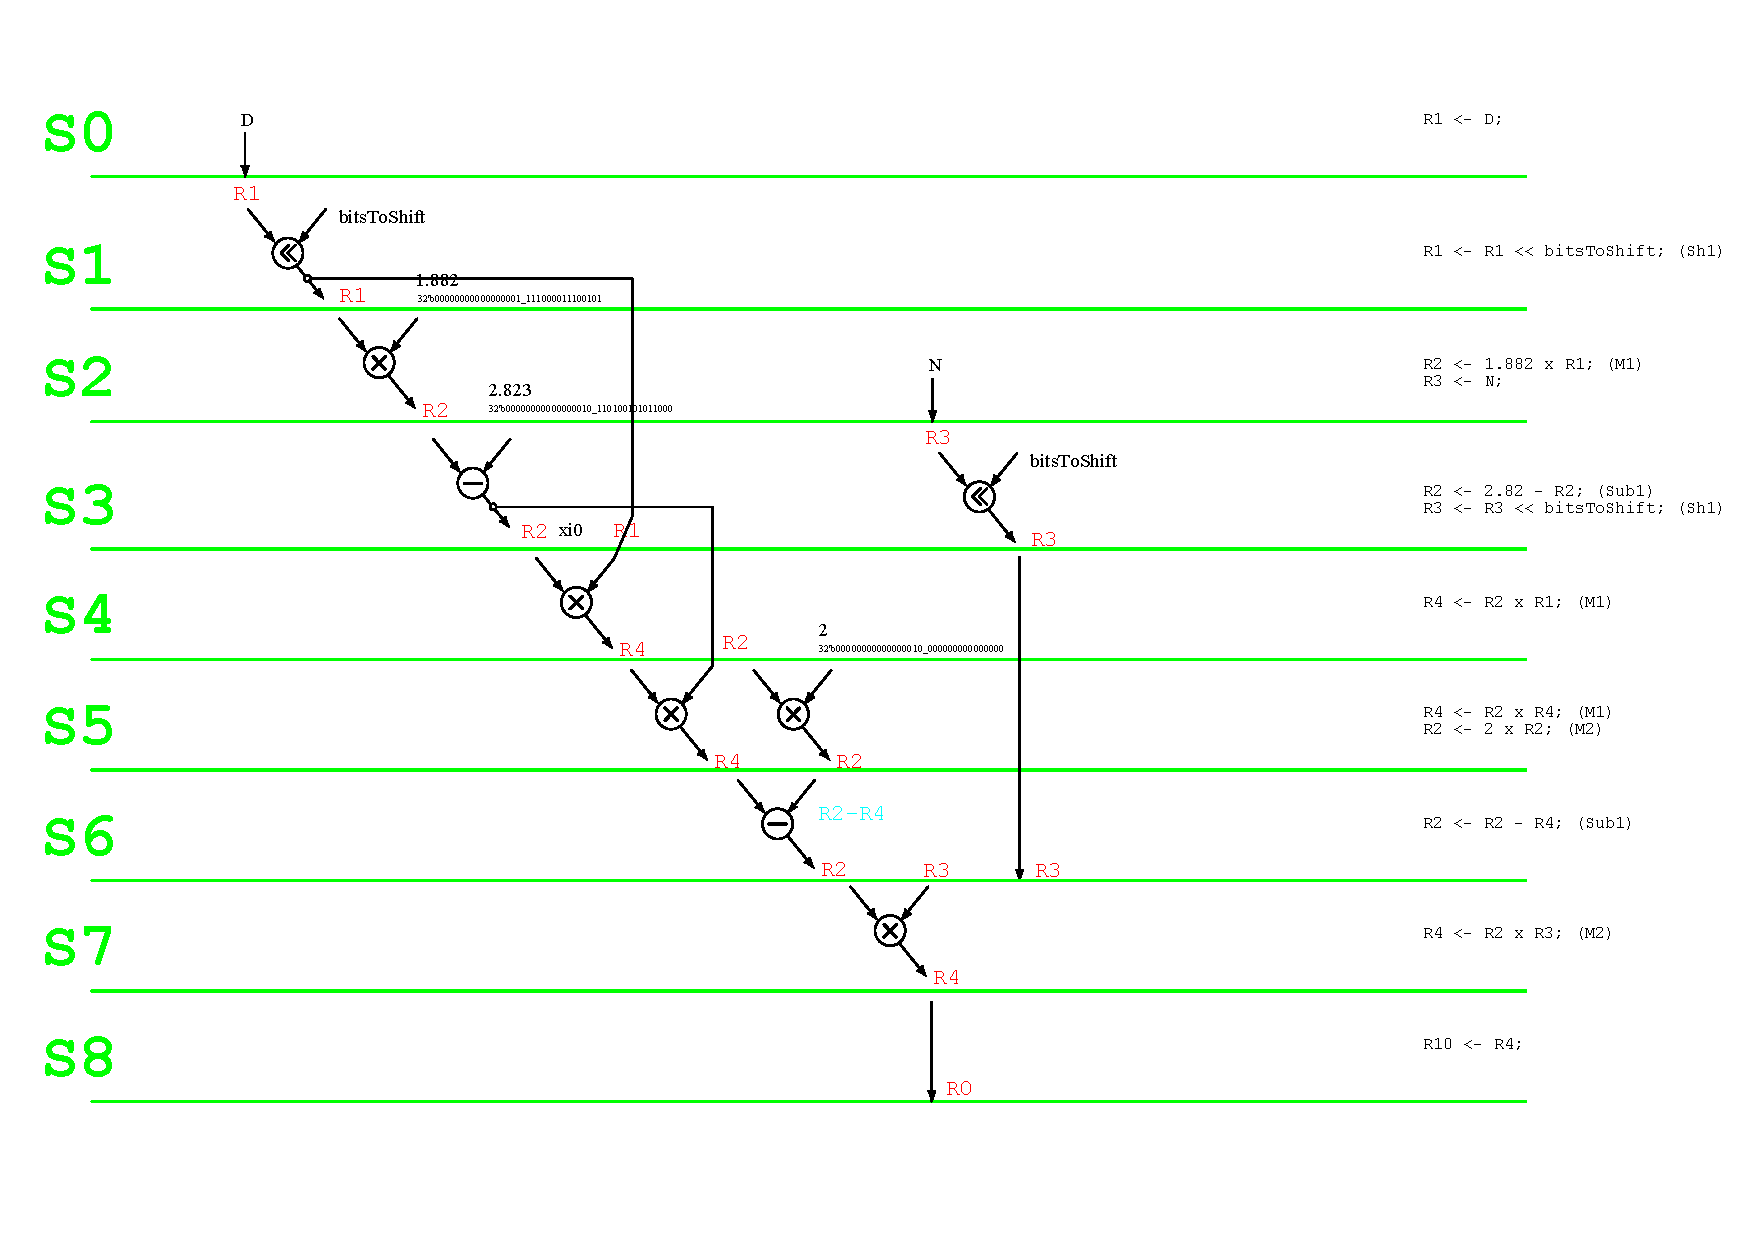
\includegraphics[width=1\textwidth]{src/pdf/allocation-timing.pdf}
   \caption{Alloccation and timing diagram for the Data Path Unit part of the \gls{abbreviation:ip}.}
  \label{fig:division-allocation-timing}
\end{figure}

\fbar
\subsubsection{Data Path Module}
The structure of created Data Path Module is depicted in the figure \ref{fig:division-rtl}. The module was specifically designed to serve the needs of the division algorithm. It consists of five registers labeled $R0$ through $R4$, two multipliers $M1$, $M2$ and one bit shifter.\par
The module si controlled by the presented control unit \gls{abbreviation:fsm} with the control signal labeled as CV. The encoding table with the labels which corresponds with the Data Path Unit module is presented in the section \hyperref[subsubsection:division-control-unit]{\textit{Control Unit}}.\par
The result of each iteration from the division algorithm is passed to a register $R0$.\par
The Data Path Module unit also covers the possibility of negative denominator and numerator. Because the values are stored in a custom \textit{Q32.15} fixed point format, the algorithm checks if the $D$ or $N$ values are higher than $0h8000$ value and determine it's actual sign and the sign if the result. If the analyzed number is determined negative, it is transformed to value positive and then used in the presented division algorithm. This transformation is needed because of the algorithm calculating the bits to shift the denominator in the interval.
\begin{figure}[htbp!]
  \centering
  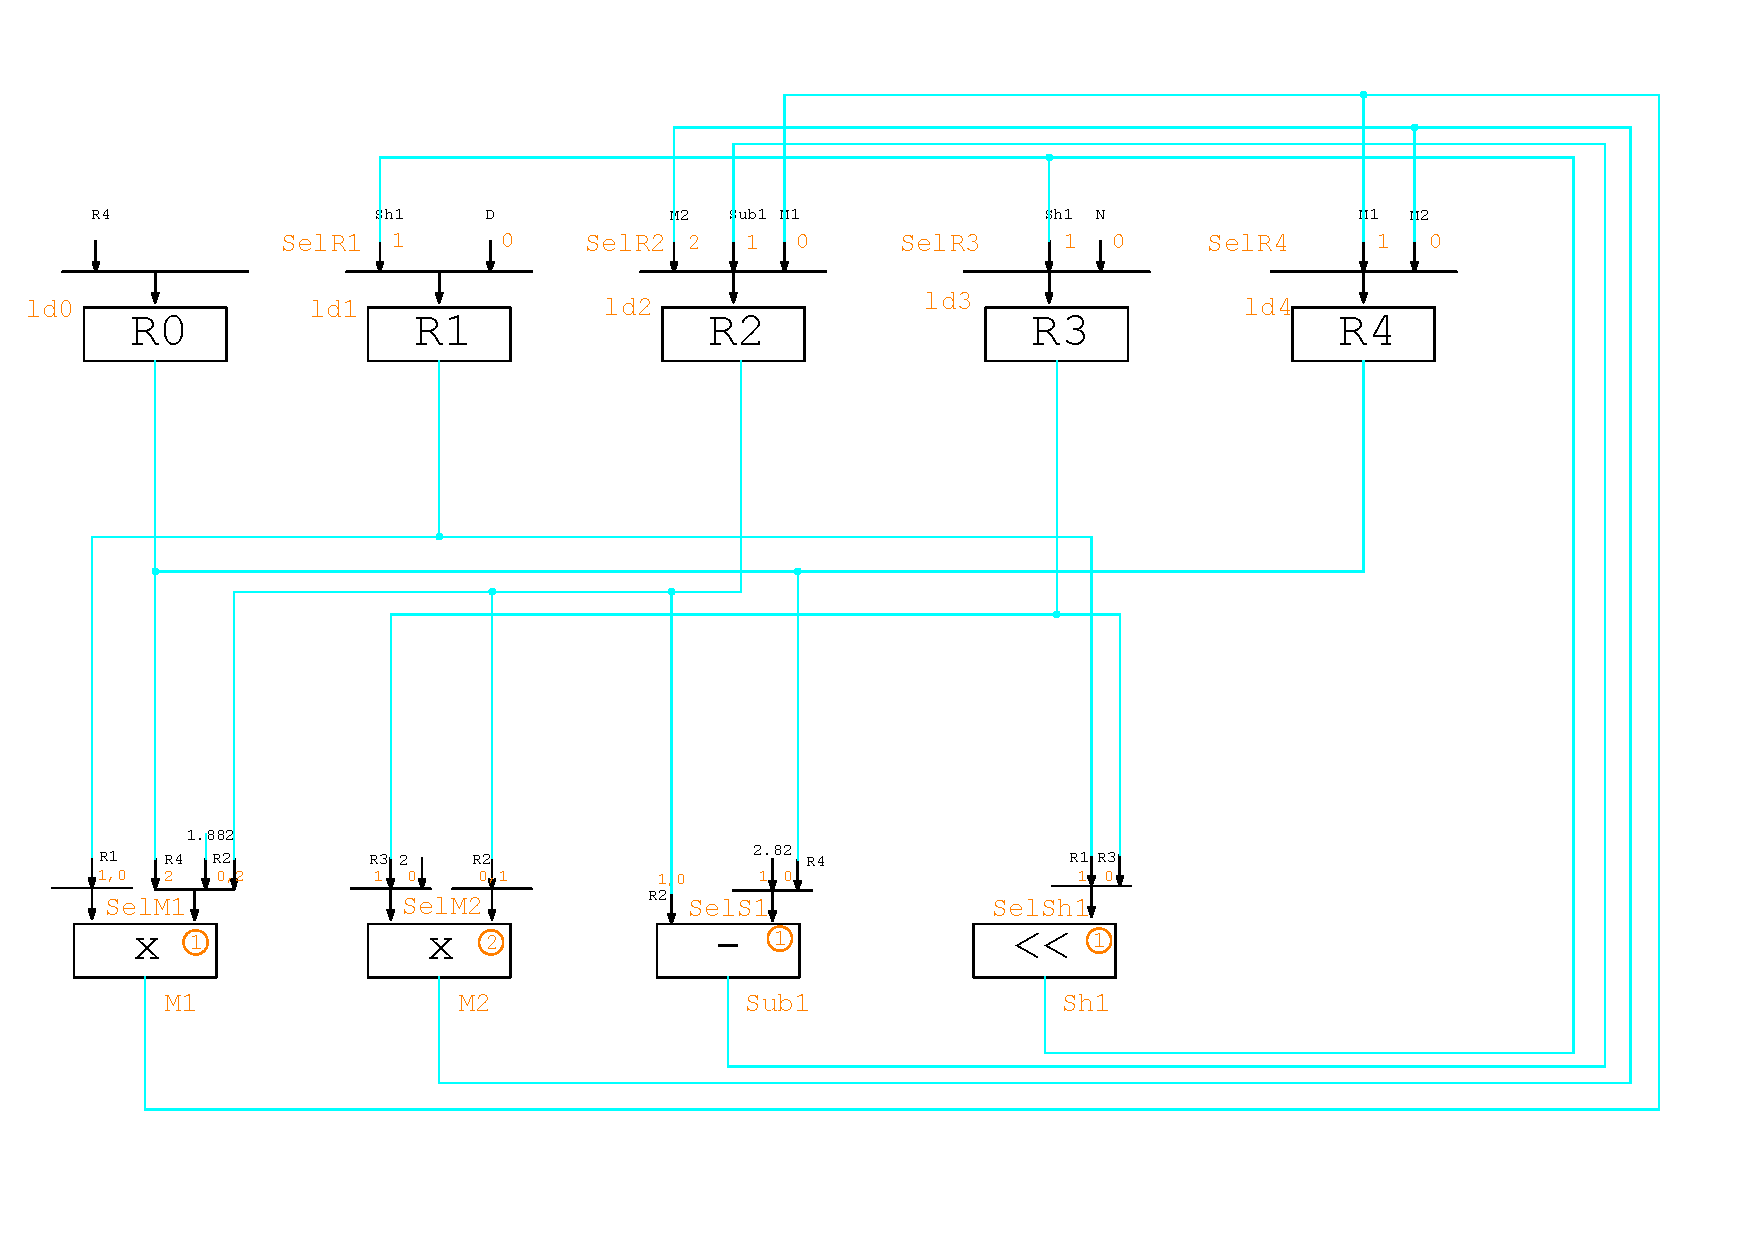
\includegraphics[width=1\textwidth]{src/pdf/rtl.pdf}
   \caption{Register transfer level \gls{abbreviation:rtl} scheme of the \gls{abbreviation:ip} Data Path Unit part of the \gls{abbreviation:ip}.}
  \label{fig:division-rtl}
\end{figure}


\fbar
\subsubsection{Control Unit}\label{subsubsection:division-control-unit}
The signals from Control Unit to Data Path Module are encoded in the CV signal. The CV signal with the corresponding instructions for the steps $S0$–$S8$ of the \gls{abbreviation:fsm} is presented in the table \ref{tab:control-signal-division-unit}. For cleaner code, the signal is passed to the Control Unit in the hexadecimal format.\par
The number of the iteration is also set in the Control Unit. The value is used in this module to determine the stop condition of the calculation.\par
As stated in the \hyperref[subsubsec:division-allocation-and-timing]{\textit{Allocation and Timing}} section, after the step \textit{S8}, the \gls{abbreviation:fsm} restarts at the state \textit{S4} with new $x_i$ values to be used in the current iteration. This jump is not depicted in the table for CV signal.
\begin{table}[htbp!]
  \centering
  \caption{Control signal encoding table for instructions to be processed by the Division Module.}
    \vspace*{0.15cm}
     \resizebox{\textwidth}{!}
    {
      \begin{tabular}{!{\vrule width 2pt} c !{\vrule width 2pt} c !{\vrule width 2pt} c  c  c !{\vrule width 2pt} c  c  c  c !{\vrule width 2pt} c  c  c  c !{\vrule width 2pt} c  c  c  c !{\vrule width 2pt} c !{\vrule width 2pt}}\noalign{\hrule height 2pt}
        \cellcolor[HTML]{B4C7DC} & \cellcolor[HTML]{B4C7DC} & \cellcolor[HTML]{5983B0}\textbf{14} & \cellcolor[HTML]{5983B0}\textbf{13} & \cellcolor[HTML]{5983B0}\textbf{12} & \cellcolor[HTML]{729FCF}\textbf{11} & \cellcolor[HTML]{729FCF}\textbf{10} & \cellcolor[HTML]{729FCF}\textbf{9} & \cellcolor[HTML]{729FCF}\textbf{8} & \cellcolor[HTML]{B4C7DC}\textbf{7} & \cellcolor[HTML]{B4C7DC}\textbf{6} & \cellcolor[HTML]{B4C7DC}\textbf{5} & \cellcolor[HTML]{B4C7DC}\textbf{4} & \cellcolor[HTML]{DEE6EF}\textbf{3} & \cellcolor[HTML]{DEE6EF}\textbf{2} & \cellcolor[HTML]{DEE6EF}\textbf{1} & \cellcolor[HTML]{DEE6EF}\textbf{0} & \multicolumn{1}{c!{\vrule width 2pt}}{\cellcolor[HTML]{FDA977}} \\
      \rowcolor[HTML]{B4C7DC} 
      \multirow{-2}{*}{\cellcolor[HTML]{B4C7DC}\textbf{State}} & \multirow{-2}{*}{\cellcolor[HTML]{B4C7DC}\textbf{RTL Code}} & \textbf{ld0} & \textbf{ld1} & \textbf{ld2} & \textbf{ld3} & \textbf{ld4} & \textbf{SelR1} & \textbf{SelR2{[}1{]}} & \textbf{SelR2{[}0{]}} & \textbf{SelR3} & \textbf{SelR4} & \textbf{SelSh1} & \textbf{SelM1{[}1{]}} & \textbf{SelM1{[}0{]}} & \textbf{SelM2} & \textbf{SelS1} & \multicolumn{1}{c!{\vrule width 2pt}}{\multirow{-2}{*}{\cellcolor[HTML]{FDA977}\textbf{CV}}} \\ \noalign{\hrule height 2pt}
      S0 & R1 ← D; & 0 & 1 & 0 & 0 & 0 & 0 & 0 & 0 & 0 & 0 & 0 & 0 & 0 & 0 & 0 & 2000h \\ \hline
      S1 & R1 ← R1\;\textless{}\textless \; 32; (Sh1) & 0 & 1 & 0 & 0 & 0 & 1 & 0 & 0 & 0 & 0 & 1 & 0 & 0 & 0 & 0 & 2210h \\ \hline
      \multirow{2}{*}{S2} & R2   ← 1.882 x R1; (M1) & \multirow{2}{*}{0} & \multirow{2}{*}{0} & \multirow{2}{*}{1} & \multirow{2}{*}{1} & \multirow{2}{*}{0} & \multirow{2}{*}{0} & \multirow{2}{*}{0} & \multirow{2}{*}{0} & \multirow{2}{*}{0} & \multirow{2}{*}{0} & \multirow{2}{*}{0} & \multirow{2}{*}{0} & \multirow{2}{*}{1} & \multirow{2}{*}{0} & \multirow{2}{*}{0} & \multirow{2}{*}{1804h} \\ 
       & R3 ← N; &  &  &  &  &  &  &  &  &  &  &  &  &  &  &  &  \\\hline
       \multirow{2}{*}{S3} & R2 ← 2.82 - R2; (Sub1) & \multirow{2}{*}{0} & \multirow{2}{*}{0} & \multirow{2}{*}{1} & \multirow{2}{*}{1} & \multirow{2}{*}{0} & \multirow{2}{*}{0} & \multirow{2}{*}{0} & \multirow{2}{*}{1} & \multirow{2}{*}{1} & \multirow{2}{*}{0} & \multirow{2}{*}{0} & \multirow{2}{*}{0} & \multirow{2}{*}{0} & \multirow{2}{*}{0} & \multirow{2}{*}{0} & \multirow{2}{*}{18C0h} \\ 
       & R3 ← R3\;\textless{}\textless\;32; (Sh1) &  &  &  &  &  &  &  &  &  &  &  &  &  &  &  &  \\\hline
      S4 & R4 ← R2 x R1; (M1) & 0 & 0 & 0 & 0 & 1 & 0 & 0 & 0 & 0 & 1 & 0 & 0 & 0 & 0 & 0 & 420h \\ \hline
       & R4 ← R2 x R4; (M1) & \multirow{2}{*}{0} & \multirow{2}{*}{0} & \multirow{2}{*}{1} & \multirow{2}{*}{0} & \multirow{2}{*}{1} & \multirow{2}{*}{0} & \multirow{2}{*}{1} & \multirow{2}{*}{0} & \multirow{2}{*}{0} & \multirow{2}{*}{1} & \multirow{2}{*}{0} & \multirow{2}{*}{1} & \multirow{2}{*}{0} & \multirow{2}{*}{0} & \multirow{2}{*}{0} & 1528h \\
      \multirow{-2}{*}{S5} & R2 ← 2 x   R2; (M2) &  &  &  &  &  &  &  &  &  &  &  &  &  &  &  &  \\ \hline
      S6 & R2 ← R2 - R4;   (S1) & 0 & 0 & 1 & 0 & 0 & 0 & 0 & 1 & 0 & 0 & 0 & 0 & 0 & 0 & 1 & 1081h \\ \hline
      S7 & R4 ← R2 x R3;   (M2) & 0 & 0 & 0 & 0 & 1 & 0 & 0 & 0 & 0 & 0 & 0 & 0 & 0 & 1 & 0 & 402h  \\ \hline
      S8 & R0 ← R4; & 1 & 0 & 0 & 0 & 0 & 0 & 0 & 0 & 0 & 0 & 0 & 0 & 0 & 0 & 0 & 4000h\\\noalign{\hrule height 2pt}
      \end{tabular}
    }
  \label{tab:control-signal-division-unit}
\end{table}
\fbar
\subsection{Calculating number of bits to shift the denominator}\label{subsec:calculating-number-of-bits-to-shift-the-denominator}
As presented in the section \hyperref[subsection:newton-raphson-algorithm-for-calculating-the-division]{\textit{Newton Rapshon algorithm for calculating the division}} the denominator must be appropriately scaled for the division algorithm to work. This section presents algorithm for scaling the denominator specified in the fixed point number format \textit{Q32.15}. After the scaling value is successfully determined, the numerator is scaled accordingly.
\par
The presented algorithm shifts the value of denominator at every positive edge of the clock signal and saves the shifted value in the \texttt{compare} register. Then the combinational circuit is utilized to compare the shifted value in \texttt{compare} register with the number \texttt{1} specified in \textit{Q32.15} format. If the compared value is the same or lower than \texttt{1} the shifting algorithm is done and the value \texttt{scaleToShift} is successfully found. If not, the inner value of shifting bits is incremented and the algorithm proceeds to the next iteration.\par
The presented algorithm is realized in the \textit{denominatorSizeScaleUnit} module and it's pseudocode is depicted in the code \ref{lst:denominatorSizeScaleUnit-pseudocode}.

\begin{lstlisting}[language={pseudocode}, caption={Pseudocode for the denominatorSizeScaleUnit module algorithm.}, label= {lst:denominatorSizeScaleUnit-pseudocode}]
  at every negative edge of clock or positive edge of reset
  if(rst)
    scaleToShift = 0;
    scaleToShiftInternal = 1;
    started = 0;
  end if
  else if (start)
  started = 1;
  end else if

  at every positive edge of clock
  if (compare <= 32'b00000000000000001_000000000000000)
  done = 1;
  started = 0;
  scaleToShift = scaleToShiftInternal;
  end if
  else
  done = 0;
  scaleToShiftInternal = scaleToShiftInternal + 1;
  end else
\end{lstlisting}

\subsection{Simulation results}
The simulation via Verilog testbench was made to determine the correctness of presented division module. The Icarus Verilog simulator was used to simulate the module and GTKWave was used to display the VCD simulation output file.\par
As for the simulation output it can be stated, that the module works correctly for positive and negative numbers of fixed point format \textit{Q32.15}.\par
The algorithm used in this module is able to calculate the propper result in much less clock cycles than the full division algorithm used in the division module in the package \cite{burke-fixed-point-math-library}.\par
Thus the presented module may be used as a submodule in more complex modules.\par
Following figures present VCD wave simulation outputs for selected $N$ and $D$. The clock frequency was set 250 MHz. Pseudocode Verilog snippet for the test bench is presented int he listing \ref{lst:division-testbench-verilog-pseudocode}. In the test bench, one unit of time corresponds to 1 ns. (based on the set timescale settings) The division unit algorithm starts at the next positive edge of clock signal after successful determination of the value \textit{bitsToShift} when the \textit{start} signal is set on low.

\begin{lstlisting}[language={pseudocode}, caption={Pseudocode snippet for the Verilog simulation test bench.}, label= {lst:division-testbench-verilog-pseudocode}]
    timescale 1ns/1ns 
    #10; // wait for 10 units of time
    #0 rstScale = 1; startScale = 0; // reset unit for determining the number of bits to shift in the denominator and do not start the unit yet
    N = 32'b00000000100110000_000010000000000; D=32'b11111111111111111_110000000000000; // set the numerator to N = 304.03125, denominator to D = -0.25
    #10 rstScale = 0; // wait for 10 units of time and stop the reset of scaling unit
    #10 startScale = 1; // start the algorithm for scaling unit
    #20 rst = 1; start = 0; // reset the division unit
    #30 rst = 0; // stop reseting of the division unit
    #20 start = 1; // start the division unit
    #20 start = 0;
    #1000; // wait 1000 units of time
    $finish; // finish the simulation
\end{lstlisting}

\begin{figure}[htbp!]
  \centering
  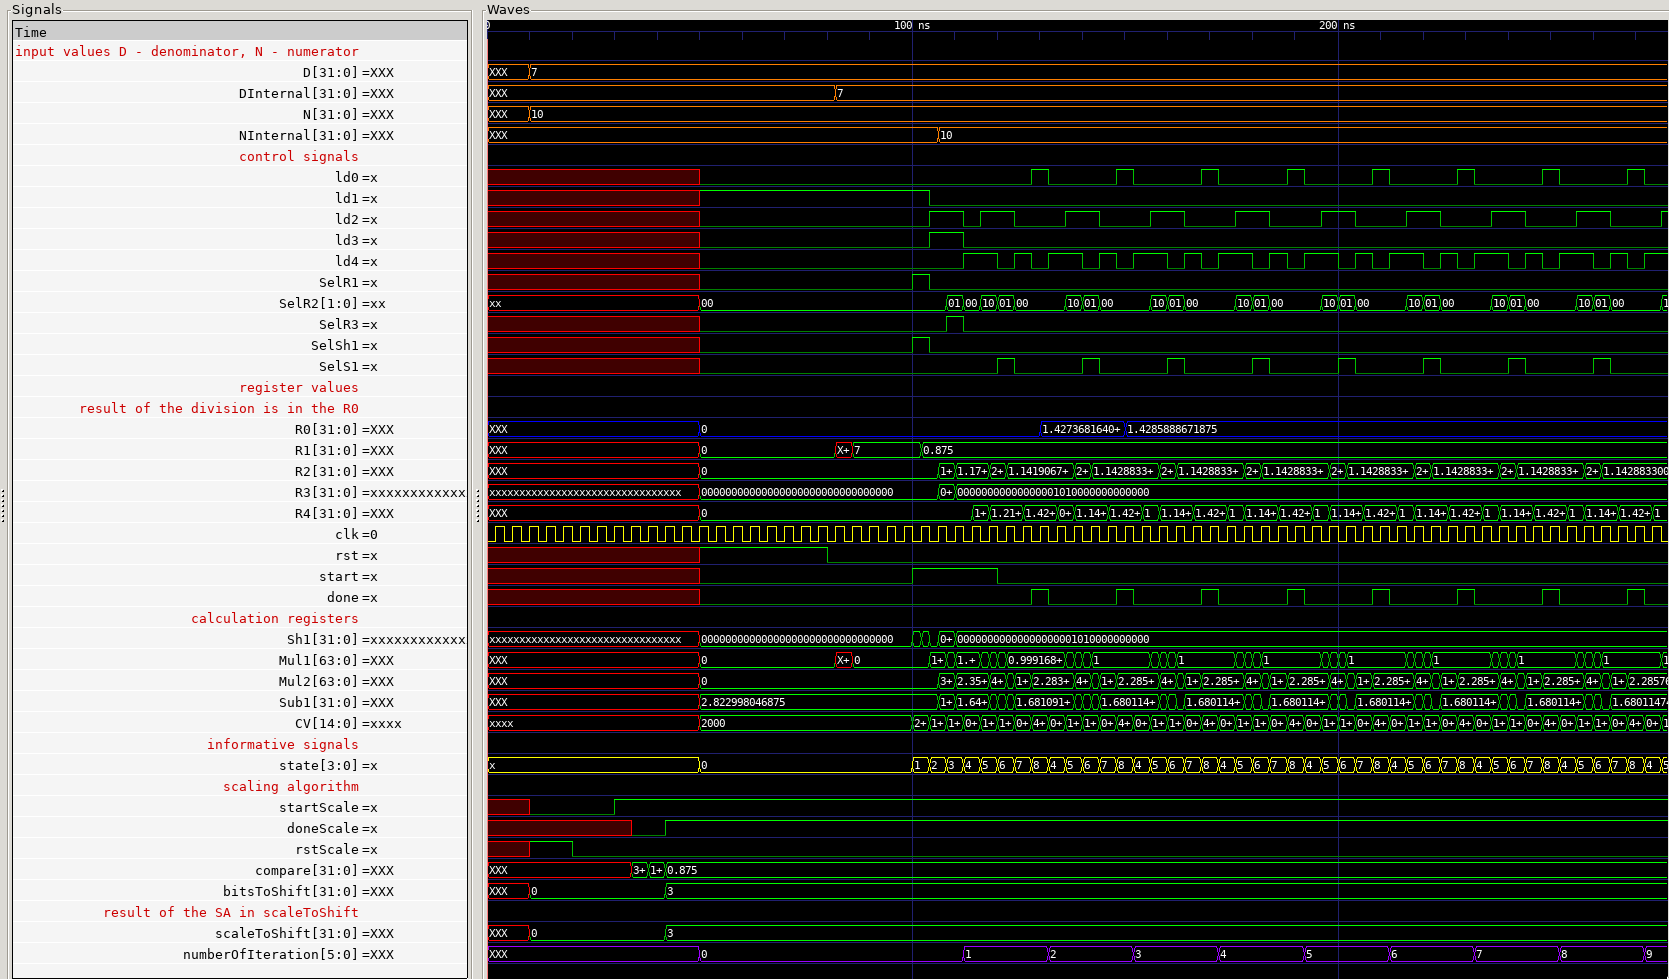
\includegraphics[width=1\textwidth]{src/png/division-10-div-7.png}
    \caption{Selected signals of simulation of division N/D = 10 / 7. The correct result in \textit{R0} is obtained after two iterations (reg numberOfIterations).}
  \label{fig:division-10-div-7}
\end{figure}


\begin{figure}[htbp!]
  \centering
  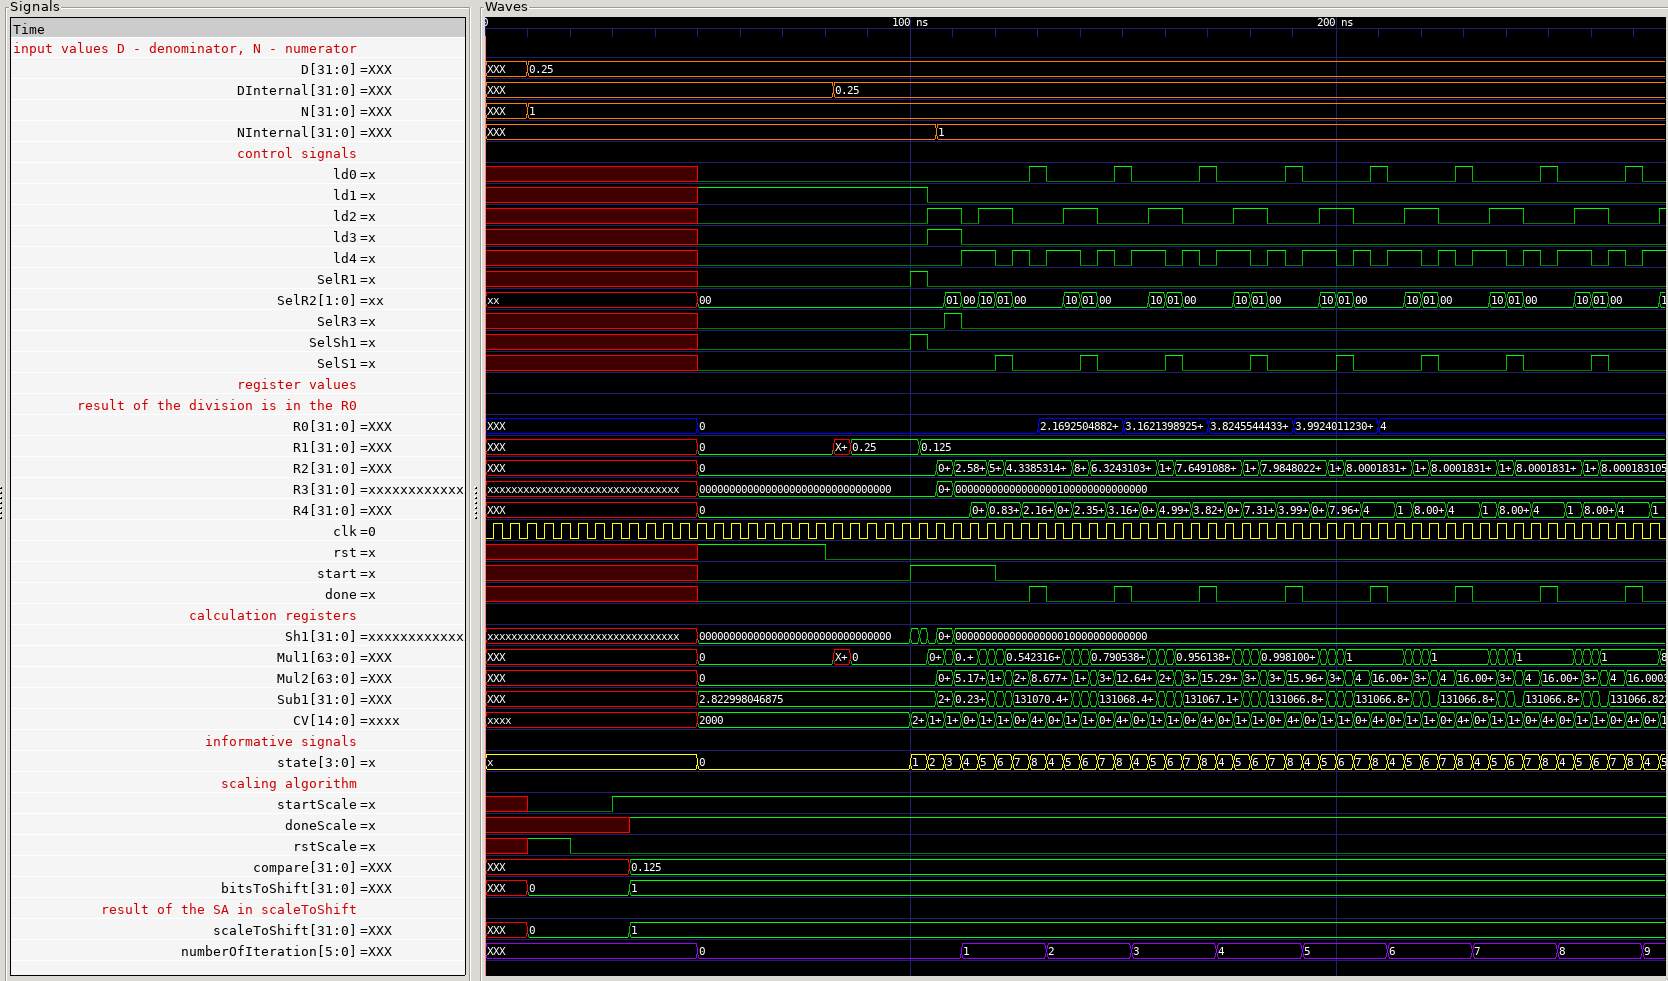
\includegraphics[width=1\textwidth]{src/png/division-1-div-0-25.png}
   \caption{Selected signals of simulation of division N/D = 1 / 0.25. The correct result in \textit{R0} is obtained after five iterations (reg numberOfIterations).}
  \label{fig:division-1-div-0-25}
\end{figure}

\begin{figure}[htbp!]
  \centering
  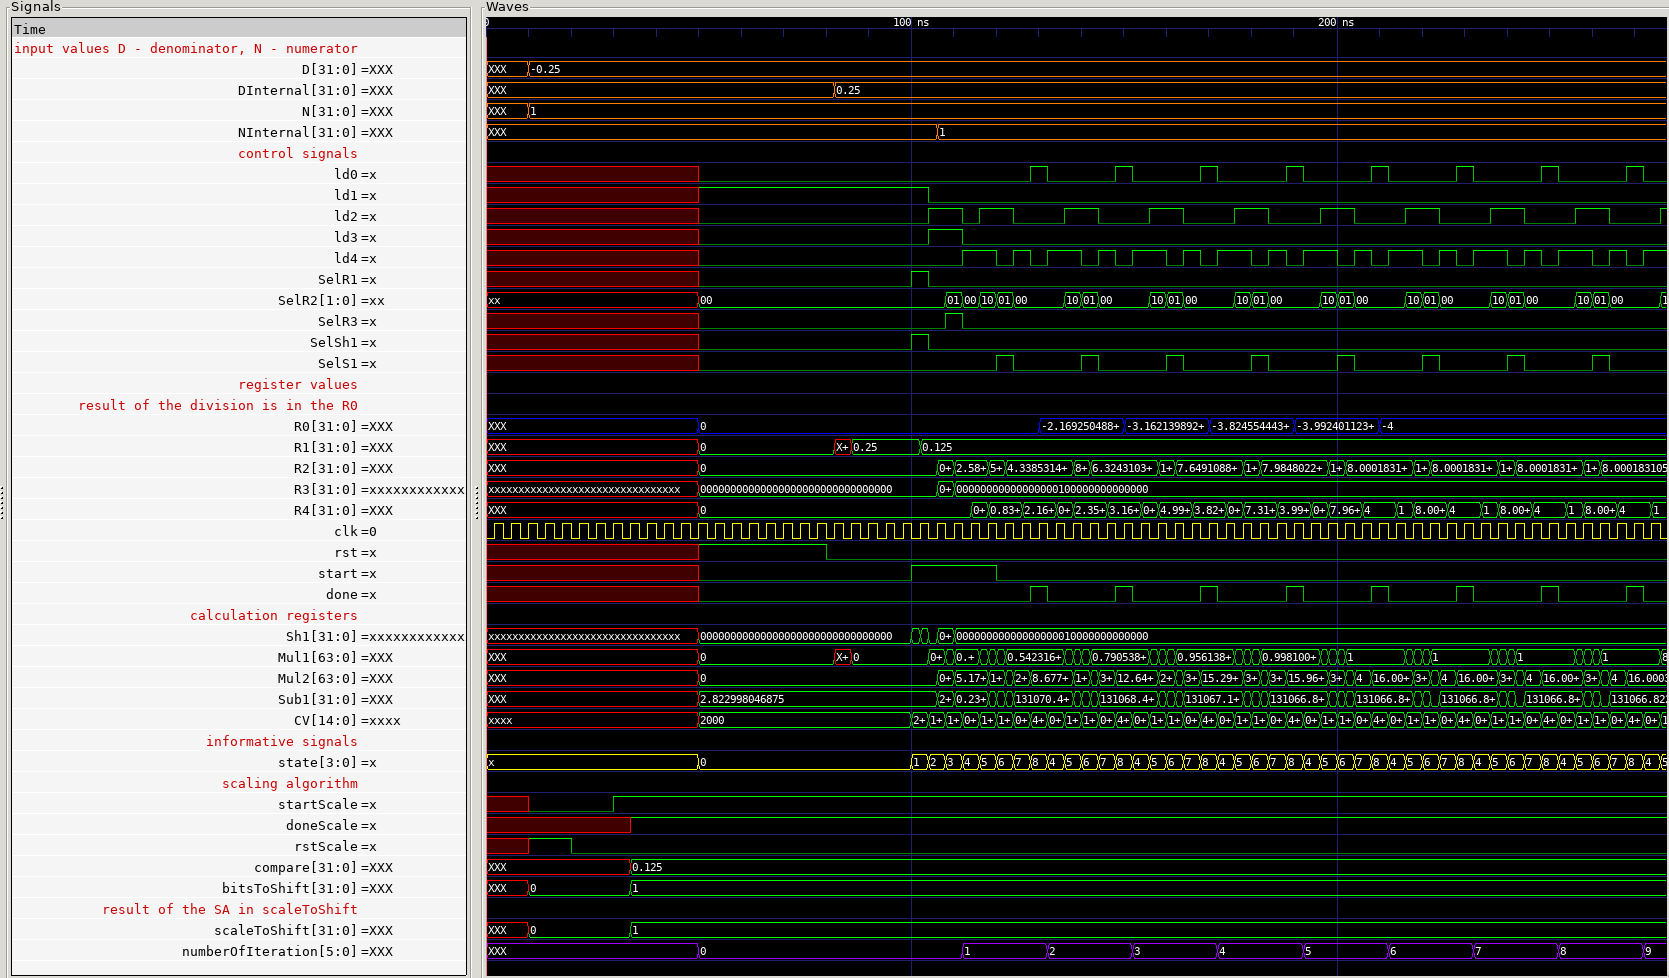
\includegraphics[width=1\textwidth]{src/png/division-1-div-minus-0-25.png}
    \caption{Selected signals of simulation of division N/D = 1 / (-0.25). The correct result in \textit{R0} is obtained after five iterations (reg numberOfIterations).}
  \label{fig:division-1-div-minus-0-25}
\end{figure}


\begin{figure}[htbp!]
  \centering
  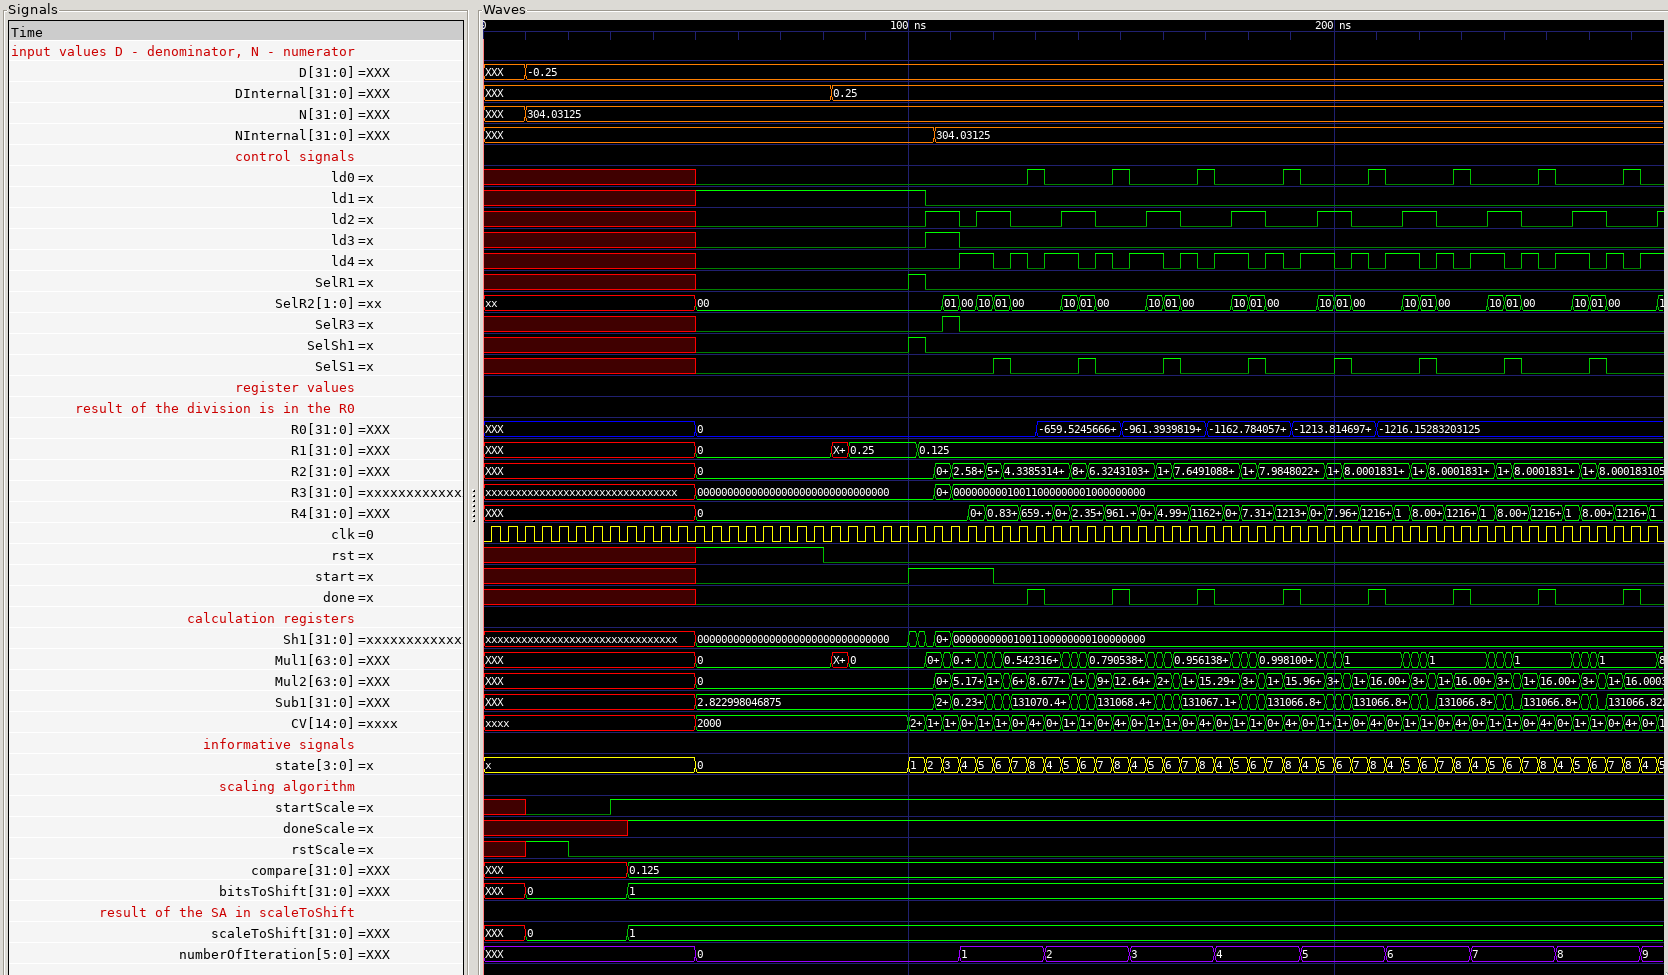
\includegraphics[width=1\textwidth]{src/png/division-304-03215-div-min-0-25.png}
    \caption{Selected signals of simulation of division N/D = 304.03215 / (-0.25). The correct result in \textit{R0} is obtained after five iterations (reg numberOfIterations).}
  \label{fig:division-304-03215-div-min-0-25}
\end{figure}

\begin{figure}[htbp!]
  \centering
  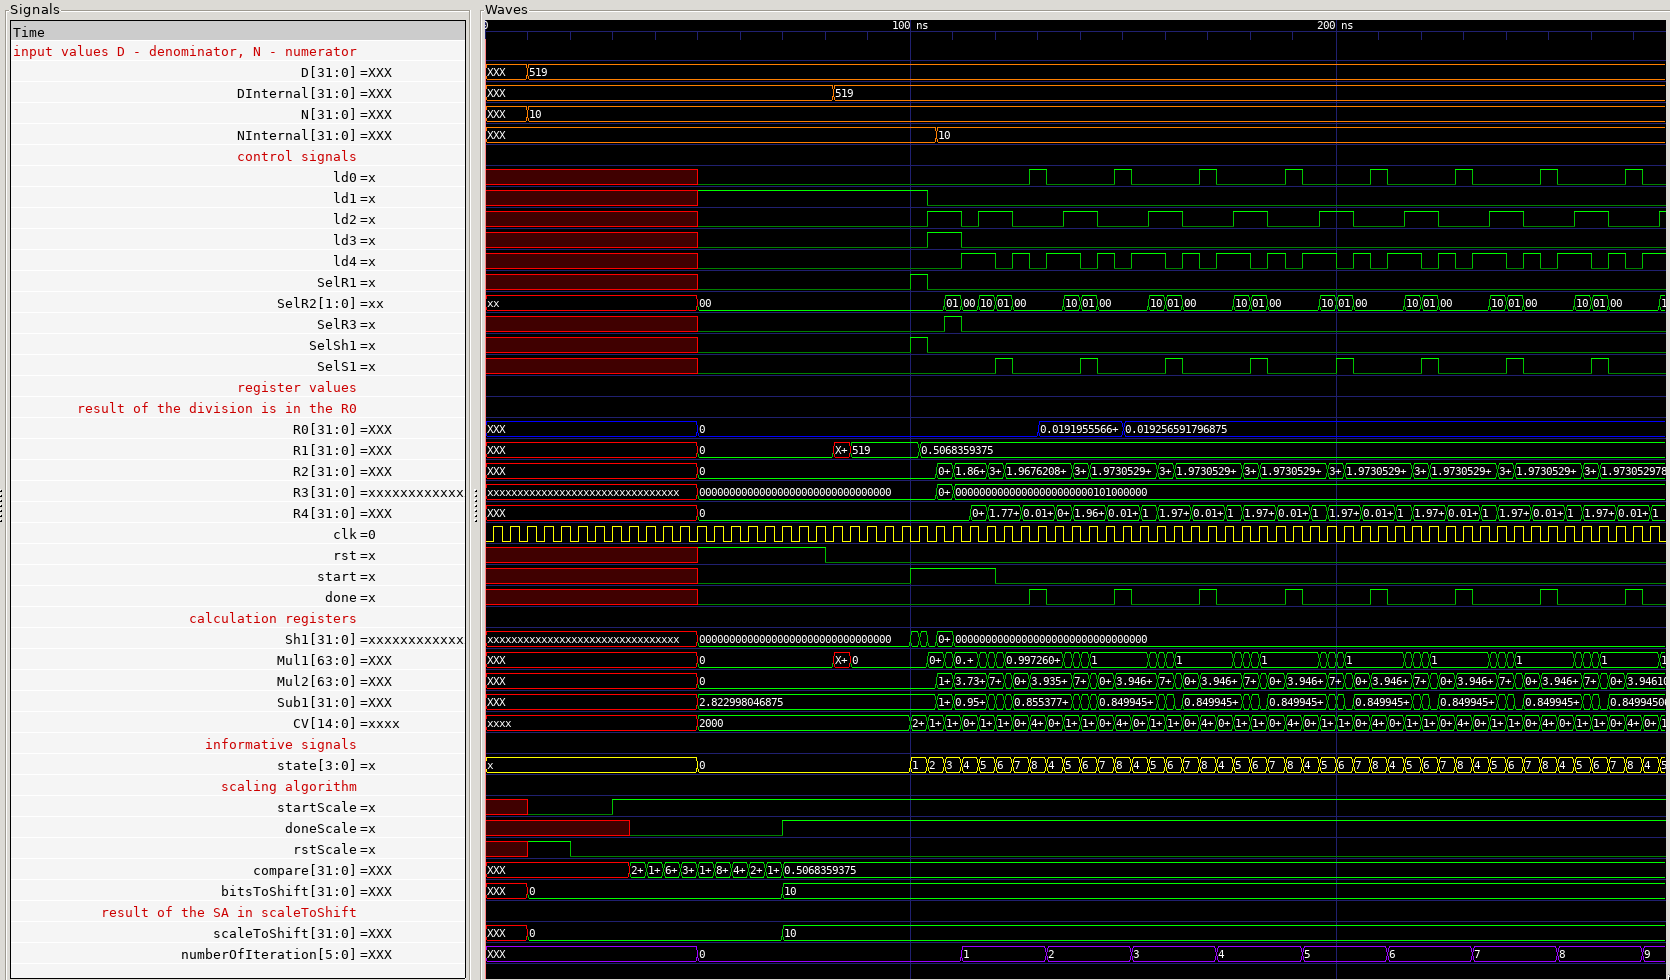
\includegraphics[width=1\textwidth]{src/png/division-10-div-519.png}
    \caption{Selected signals of simulation of division N/D = 10 / (519). The correct result in \textit{R0} is obtained after two iterations (reg numberOfIterations).}
  \label{fig:division-10-div-519}
\end{figure}

\section{Using CORDIC to calculate trigonometric functions}
    There are few approaches when there is a need to calculate the trigonometric functions. In this work, the \gls{abbreviation:cordic} was used. To get more flexibility in the calculation the implementation of \gls{abbreviation:cordic} algorithm was chosen above the \gls{abbreviation:lut} for calculation.\par
    The \gls{abbreviation:lut} method may be fast, but the accuracy depends on the size of the table. When using the \gls{abbreviation:cordic} one can influence the precision by using more iterations of the algorithm. The modified algorithm may be used to calculate non-trivial functions, such as hyperbolic functions, square roots, multiplications, divisions, exponentials and logarithms. \cite{base-digital-signal-processing-with-field-programmable-gate-arrays} In this work only the calculation of $sinus$ and $cosinus$ functions is used.
    \subsection{Theory}
        The theory of the first \gls{abbreviation:cordic} was proposed by Volder in \cite{volder-cordic-trigonomtric-computing-technique}. This algorithm computes a coordinate conversion between rectangular ($x$, $y$) and polar ($R$, $\theta$) coordinates. The algorithm was then generalized by Walther in \cite{walther-a-unified-algorithm-for-elementary-functions} to include circular, linear and hyperbolic transforms. This paper utilizes only circular transforms to calculate $sinus$ and $cosinus$ functions. Only the most basic approach to the algorithm will be presented.\par
        The rotation of a vector in the rectangular coordinate system ($x$, $y$) may be described by matrix-vector multiplication depicted in the eq. \ref{eq:rotation}.

        \begin{equation}\label{eq:rotation}
             \begin{pmatrix}
                 x_\text{R}\\
                 y_\text{R}
             \end{pmatrix}
             =
             \begin{pmatrix}
                 \cos (\theta) & -\sin (\theta)\\
                 \sin (\theta) & \cos (\theta)
             \end{pmatrix}
             \begin{pmatrix}
                 x_\text{in}\\
                 y_\text{in}
             \end{pmatrix},
        \end{equation}

        where $x_\text{R}$ and $y_\text{R}$ are coordinates of a rotated vector, $\theta$ is the angle for which the vector with coordinates $x_\text{in}$ and $y_\text{in}$ was rotated.\par
        Then when simplifying the equation


        \begin{equation}\label{eq:rotation-simplifying}
             \begin{pmatrix}
                 x_\text{R}\\
                 y_\text{R}
             \end{pmatrix}
             = \cos (\theta)
             \begin{pmatrix}
                 1 & -\tan (\theta)\\
                 \tan (\theta) & 1
             \end{pmatrix}
             \begin{pmatrix}
                 x_\text{in}\\
                 y_\text{in}
             \end{pmatrix}
        \end{equation}

        it can be seen, that only multiplication by scaling factor of precalculated values of $\cos (\theta)$, multiplication by $\tan (\theta)$, subtraction and addiction operations are needed. However, the multiplication by $\tan (\theta)$ can be interchanged. The interchange may be done for angles $\theta$ for which the equation \ref{eq:tan-theta-2} is true. The when implementing the algorithm to the \gls{abbreviation:fpga} the multiplication may be swapped for signed right bit shift.

        \begin{equation}\label{eq:tan-theta-2}
            \tan (\theta) = 2^{-1}.
        \end{equation}
        \par
        Then when the values $x_\text{in} = 1$ and $y_\text{in} = 0$ are used, the result for $sinus$ and $cosinus$ can be easily obtained from $x_\text{R}$ and $y_\text{R}$ as expressed in the equation \ref{eq:xr-yr-when-initial-values-1-0}.

        \begin{equation}\label{eq:xr-yr-when-initial-values-1-0}
            x_\text{R} = x_\text{in} \cos (\theta) - y_\text{in} \sin (\theta) = | \theta = 0 | = \cos (\theta)
            y_\text{R} = x_\text{in} \sin (\theta) + y_\text{in} \cos (\theta) = | \theta = 0 | = \sin (\theta)
        \end{equation}

            The algorithm may be further simplified by expecting that the algorithm is designed to use more than 6 iterations and thus the scaling constant represented by multipliying $cosinus$ of different $\theta$ values converges to $0,60725$. So there is no need to precalculate all the scaling values and use only the value of the convergence. In this paper the scaling values are precalculated and passed from the custom \gls{abbreviation:lut} module.\par
            As can be seen from the section \hyperref[subsubsec:example-of-calculation]{\textit{Example of calculation}} section or the algortihm teory itself, it needs to be determined, if the angle for which the vector is rotated in the next iteration should be in a positive direction (counter-clockwise) or negative direction (clockwise). For that, the set of the equations is expanded with value $z_i$. The complete set of equations which are used in the \hyperref[subsec:cordic-implementation]{\textit{Implementation}} are as follows.

            \begin{equation}
                \begin{gathered}
                x [i+1] = x [i] - \sigma_i 2^{-i} y[i],\\
                y [i+1] = y [i] + \sigma_i 2^{-i} x[i],\\
                z~[i+1] = z~[i] - \sigma_i \atan (2^{-i}).
                \end{gathered}
            \end{equation}
            The $\sigma_{i+1}$ is determined based on the sign of the $z_{i+1}$ variable

            \begin{equation}
                \sigma_{i+1} = 
                \left\{
                \begin{array}{lr}
                    -1,\;\text{if}\;z_{i+1} < 0\\
                    1,\;\text{if}\;z_{i+1} > 0\\
                    0,\;\text{if}\;z_{i+1} = 0
                \end{array}
                \right\}
            \end{equation}
            \par
            The algorithm as presented calculates the correct values for $sinus$ and $cosinus$ functions only in the first and fourth quadrant ($3\pi/2$ to $\pi/2$ counter-clockwise). For usage of the whole $2\pi$ range, corresponding actions before the 0. iteration must be made.\par
            The algorithm must make checks, to determine the quadrant, where the desired angle $\theta$ for which the $sinus$ and $cosinus$ functions are to be calculated. This is done by \texttt{if} statements at the algorithm values initialization and at the final function value calculation. If the desired argument of the functions is not in the first or fourth quadrant then the angle is transfered from the actual quadrant to the first or fourth quadrant. Based on the quadrant, to which the angle is transformed, the $\sigma_i$ value is set. The corresponding if statements a the algorithm initialization are presented in the pseudocode \ref{lst:cordic-initial-if-statements}.\par
            Similar if statements are used at the final calculation of $sinus$ and $cosinus$ values. The if statements are presented in the pseudocode \ref{lst:cordic-ending-if-statements}.\par
            The pseudocodes use \texttt{initialZValue} as a desired angle $\theta$, for which to calculate the function values, \texttt{zValue} as a temporary value for calculating the iterations for $z_{i}$ variables, \texttt{sigmaValue} for temporary value holding the current iteration value of $\sigma_i$, the \texttt{resultCos} and \texttt{resultSin} variables are used for storing the temporary and final values of the $\cos (\theta)$ and $\sin (\theta)$ values respectively.

\begin{lstlisting}[language={pseudocode}, caption={Pseudocode for if statements used at the value initialization of the \gls{abbreviation:cordic} algorithm.}, label= {lst:cordic-initial-if-statements}]
if((initialZValue > 1.5707)&(initialZValue < 3.141592))
    sigmaValue = -1
    zValue = initialZValue - 3.141592
else if((initialZValue > 3.141592)&(initialZValue < 4.7123))
    sigmaValue = 1
    zValue = initialZValue - 3.141592
else
    zValue = initialZValue
    sigmaValue = 1
end
\end{lstlisting}


\begin{lstlisting}[language={pseudocode}, caption={Pseudocode for if statements used at the final $sinus$ and $cosinus$ value calculation.}, label= {lst:cordic-ending-if-statements}]
if((initialZValue > 1.5707)&(initialZValue < 3.141592))
    resultCos = - resultCos
    resultSin = resultSin
else if((initialZValue > 3.141592)&(initialZValue < 4.7123))
    resultCos = - resultCos
    resultSin = - resultSin
end
\end{lstlisting}

        \subsubsection{Example of calculation}\label{subsubsec:example-of-calculation}
            The general approach of \gls{abbreviation:cordic} algorithm may be explained on the example for calculating the $sinus$ and $cosinus$ values for the angle $\theta = 57,535\;˚$. Firstly, the angle may be destructurized in the base angles, for which the equation \ref{eq:tan-theta-2} is true. In this example the is destructurized as $57,535 = 45 + 25,565 -14,03$.\par
            The index $i$ of the variables $x_i$ and $y_i$ in the following equations means the number of iteration of the algorithm.

            \begin{equation}
                0.\;\text{iteration}\;
                \begin{pmatrix}
                    x_0\\y_0
                \end{pmatrix}
                =
                \cos (45\;°)
                \begin{pmatrix}
                    1 & -1\\
                    1 & 1
                \end{pmatrix}
                \begin{pmatrix}
                    x_\text{in}\\
                    y_\text{in}
                \end{pmatrix},
            \end{equation}

            
            \begin{equation}
                1.\;\text{iteration}\;
                \begin{pmatrix}
                    x_1\\y_1
                \end{pmatrix}
                =
                \cos (26,565\;°)
                \begin{pmatrix}
                    1 & -2^{-1}\\
                    2^{-1} & 1
                \end{pmatrix}
                \begin{pmatrix}
                    x_0\\
                    y_0
                \end{pmatrix},
            \end{equation}


            \begin{equation}
                2.\;\text{iteration}\;
                \begin{pmatrix}
                    x_2\\y_2
                \end{pmatrix}
                =
                \cos (-14,03\;°)
                \begin{pmatrix}
                    1 & -2^{-2}\\
                    2^{-2} & 1
                \end{pmatrix}
                \begin{pmatrix}
                    x_1\\
                    y_1
                \end{pmatrix}.
            \end{equation}

            Then after substitution the value of $x_2$ and $y_2$ may be obtained.\par
            \begin{equation}\label{eq:example-cordic-calculation}
                \begin{pmatrix}
                    x_2\\y_2
                \end{pmatrix}
                =
                \cos (45\;°)
                \cos (25,565\;°)
                \cos (-14,03\;°)
                \begin{pmatrix}
                    1 & -2^{-2}\\
                    2^{-2} & 1
                \end{pmatrix}
                \begin{pmatrix}
                    1 & -2^{-1}\\
                    2^{-1} & 1
                \end{pmatrix}
                \begin{pmatrix}
                    1 & -1\\
                    1 & 1
                \end{pmatrix}
                \begin{pmatrix}
                    x_\text{in}\\
                    y_\text{in}
                \end{pmatrix}.
            \end{equation}

            \par
            From the equation \ref{eq:example-cordic-calculation} the values $x_2$ and $y_2$ represent the value of $\cos (57,535\;˚)$ and $\sin (57,535\;˚)$ respectively.

    \subsection{Implementation}\label{subsec:cordic-implementation}
        The \gls{abbreviation:cordic} algorithm was for simplicity prototyped in python. This turned out very beneficial as the debugging of the code is much faster. The less complex and abstract python code may help with understanding and creating the designed algorithms more than Mathematica which uses some higher abstraction layers to make calculations optimized and easier for more complex problems. But when designing the low level mathematical algorithms, the lower and easier language the more easy is then to implement the design in Verilog or any other hardware description language.\par
        The python code was as well used to precalculate the \gls{abbreviation:lut} for scaling factor and arcus tangens values for $z_i$ calculations.\par
        For the clarity, the python implementation is presented in the code \ref{lst:python-cordic}. The code also calculates the error of the \gls{abbreviation:cordic} calculated value from the python math library functions.

\begin{lstlisting}[language={python}, caption={Python code of \gls{abbreviation:cordic} implementation.}, label= {lst:python-cordic}]
import math

# Defining starting values and empty arrays
totalNumberOfIterations = 12 # 12 - best tradeof between value and iterations
atanValues = []
scalingValues = [1]
initialXValueCordic = 1
initialYValueCordic = 0
initialZValueCordic = - 1.248  # angle for which to calculate cordic
initialSigmaValueCordic = 1

for x in range(totalNumberOfIterations):
    # Generating arcus tanges values of precalculated angles based on number of iterations
    atanValues.append(math.atan(1*2**(-x)))
    # Generating precalculated scaling values based on a number of iterations
    scalingValues.append(scalingValues[x]*math.cos(atanValues[x]))

print("atanValues: ", atanValues)
print("scalingValues: ", scalingValues)


# Checking the initial value and moving it in the interval
if (initialZValueCordic > 1.5707) and (initialZValueCordic < 3.141592):
    zValue = initialZValueCordic - 3.141592
    sigmaValue = -1
    print("value in second q")
elif (initialZValueCordic > 3.141592) and (initialZValueCordic < 4.7123):
    zValue = initialZValueCordic - 3.141592
    sigmaValue = 1
    print("value in third q")
elif (initialZValueCordic < 0):
    sigmaValue = -1
    zValue = initialZValueCordic
    print("value in fourth q")
else:
    zValue = initialZValueCordic  # For angle
    sigmaValue = initialSigmaValueCordic  # For +- next angle
    print("value in first")

# Passing starting values to the calculation values
xValue = initialXValueCordic  # For cos
yValue = initialYValueCordic  # For sin


# CORDIC ALGORITHM
for x in range(totalNumberOfIterations):

    # Calculating next values of the current iteration x
    xNextValue = xValue - (sigmaValue*yValue)*2**(-x)
    yNextValue = yValue + (sigmaValue*xValue)*2**(-x)
    zNextValue = zValue - sigmaValue * atanValues[x]

    # Determining the signum of next angle (addition or subtraction)
    if zNextValue >= 0:
        sigmaNextValue = 1
    else:
        sigmaNextValue = -1

    # Values for new iteration
    xValue = xNextValue
    yValue = yNextValue
    zValue = zNextValue
    sigmaValue = sigmaNextValue

    print("iteration:", x, "xValue:", xValue, "yValue:", yValue, "zValue:", zValue, "sigmaValue:", sigmaValue, "\n")

# Calculating results by scaling the result values from CORDIC by the scalingValue which depends on number of iterations which were made
resultCos = scalingValues[x-1] * xValue
resultSin = scalingValues[x-1] * yValue

# Changing results sign based on the rotation of the initialZValueCordic
if (initialZValueCordic > 1.5707) and (initialZValueCordic < 3.141592):
    resultCos = - resultCos
elif (initialZValueCordic > 3.141592) and (initialZValueCordic < 4.7123):
    resultCos = - resultCos
    resultSin = - resultSin

#Calculating values based on the math library
mathResultCos = math.cos(initialZValueCordic)
mathResultSin = math.sin(initialZValueCordic)

# Calculating the error of CORDIC calculated values from the python math functions
errorCos = abs(resultCos) - abs(mathResultCos)
errorSin = abs(resultSin) - abs(mathResultSin)
\end{lstlisting}

\par
After the python implementation and debugging has been finalized, the circuit Verilog implementation of the algorithm could be initiated. Same as for the Division Unit IP, presented in \hyperref[sec:calculating-the-division-of-fixed-point-numbers]{\textit{Calculating the division of fixed point numbers}} section, the Data Path, Control Unit and Top Module was designed. This approach based on the application specific circuit design should be by its nature faster and more safe than creating the custom \gls{abbreviation:cpu} with reduced and customized \gls{abbreviation:isa}.

    \subsubsection{Control Unit}
        
        \begin{table}[htbp!]
            \centering
            \caption{Control signal encoding table for instructions to be processed by the Division Module.}
            \vspace*{0.15cm}
            \resizebox{\textwidth}{!}
                {
\begin{tabular}{!{\vrule width 2pt} c !{\vrule width 2pt} l !{\vrule width 2pt} c c c !{\vrule width 2pt} c  c c  c !{\vrule width 2pt} c c c c !{\vrule width 2pt} c c c c !{\vrule width 2pt} c c c c !{\vrule width 2pt} c c c c !{\vrule width 2pt} c !{\vrule width 2pt}}\noalign{\hrule height 2pt}
\cellcolor[HTML]{B4C7DC}  & \cellcolor[HTML]{B4C7DC}                                                          & \cellcolor[HTML]{355269}{\color[HTML]{FFFFFF} \textbf{22}}  & \cellcolor[HTML]{355269}{\color[HTML]{FFFFFF} \textbf{21}}  & \cellcolor[HTML]{355269}{\color[HTML]{FFFFFF} \textbf{20}}  & \cellcolor[HTML]{3465A4}{\color[HTML]{FFFFFF} \textbf{19}}  & \cellcolor[HTML]{3465A4}{\color[HTML]{FFFFFF} \textbf{18}}  & \cellcolor[HTML]{3465A4}{\color[HTML]{FFFFFF} \textbf{17}}  & \cellcolor[HTML]{3465A4}{\color[HTML]{FFFFFF} \textbf{16}}  & \cellcolor[HTML]{5983B0}\textbf{15}         & \cellcolor[HTML]{5983B0}\textbf{14}         & \cellcolor[HTML]{5983B0}\textbf{13}         & \cellcolor[HTML]{5983B0}\textbf{12}         & \cellcolor[HTML]{729FCF}\textbf{11}         & \cellcolor[HTML]{729FCF}\textbf{10}           & \cellcolor[HTML]{729FCF}\textbf{9}            & \cellcolor[HTML]{729FCF}\textbf{8}          & \cellcolor[HTML]{B4C7DC}\textbf{7}          & \cellcolor[HTML]{B4C7DC}\textbf{6}          & \cellcolor[HTML]{B4C7DC}\textbf{5}          & \cellcolor[HTML]{B4C7DC}\textbf{4}          & \cellcolor[HTML]{DEE6EF}\textbf{3}          & \cellcolor[HTML]{DEE6EF}\textbf{2}          & \cellcolor[HTML]{DEE6EF}\textbf{1}          & \cellcolor[HTML]{DEE6EF}\textbf{0}          & \cellcolor[HTML]{FDA978}                              \\
    \multirow{-2}{*}{\cellcolor[HTML]{B4C7DC}\textbf{State}} & \multirow{-2}{*}{\cellcolor[HTML]{B4C7DC}\textbf{RTL Code}}                       & \cellcolor[HTML]{355269}{\color[HTML]{FFFFFF} \textbf{ld1}} & \cellcolor[HTML]{355269}{\color[HTML]{FFFFFF} \textbf{ld2}} & \cellcolor[HTML]{355269}{\color[HTML]{FFFFFF} \textbf{ld3}} & \cellcolor[HTML]{3465A4}{\color[HTML]{FFFFFF} \textbf{ld4}} & \cellcolor[HTML]{3465A4}{\color[HTML]{FFFFFF} \textbf{ld5}} & \cellcolor[HTML]{3465A4}{\color[HTML]{FFFFFF} \textbf{ld6}} & \cellcolor[HTML]{3465A4}{\color[HTML]{FFFFFF} \textbf{ld7}} & \cellcolor[HTML]{5983B0}\textbf{ld8}        & \cellcolor[HTML]{5983B0}\textbf{ld9}        & \cellcolor[HTML]{5983B0}\textbf{ld10}       & \cellcolor[HTML]{5983B0}\textbf{SelR1}      & \cellcolor[HTML]{729FCF}\textbf{SelR2}      & \cellcolor[HTML]{729FCF}\textbf{SelR4{[}1{]}} & \cellcolor[HTML]{729FCF}\textbf{SelR4{[}0{]}} & \cellcolor[HTML]{729FCF}\textbf{SelR5}      & \cellcolor[HTML]{B4C7DC}\textbf{SelR6}      & \cellcolor[HTML]{B4C7DC}\textbf{SelR7}      & \cellcolor[HTML]{B4C7DC}\textbf{SelR9}      & \cellcolor[HTML]{B4C7DC}\textbf{SelR10}     & \cellcolor[HTML]{DEE6EF}\textbf{SelM1}      & \cellcolor[HTML]{DEE6EF}\textbf{SelM2}      & \cellcolor[HTML]{DEE6EF}\textbf{SelSub1}    & \cellcolor[HTML]{DEE6EF}\textbf{SelSub2}    & \multirow{-2}{*}{\cellcolor[HTML]{FDA978}\textbf{CV}} \\!{\vrule width 2pt}
                                       & R0 ← totalNumberOfIterations;                                                     &                                                             &                                                             &                                                             &                                                             &                                                             &                                                             &                                                             &                                             &                                             &                                             &                                             &                                             &                                               &                                               &                                             &                                             &                                             &                                             &                                             &                                             &                                             &                                             &                                             &                                                       \\
                                       & R1 ← initialXValue;                                                               &                                                             &                                                             &                                                             &                                                             &                                                             &                                                             &                                                             &                                             &                                             &                                             &                                             &                                             &                                               &                                               &                                             &                                             &                                             &                                             &                                             &                                             &                                             &                                             &                                             &                                                       \\
                                       & R2 ← initialYValue;                                                               &                                                             &                                                             &                                                             &                                                             &                                                             &                                                             &                                                             &                                             &                                             &                                             &                                             &                                             &                                               &                                               &                                             &                                             &                                             &                                             &                                             &                                             &                                             &                                             &                                             &                                                       \\
\multirow{-4}{*}{S0}                   & R3 ← initialZValue;                                                               & \multirow{-4}{*}{1}                                         & \multirow{-4}{*}{1}                                         & \multirow{-4}{*}{1}                                         & \multirow{-4}{*}{0}                                         & \multirow{-4}{*}{0}                                         & \multirow{-4}{*}{0}                                         & \multirow{-4}{*}{0}                                         & \multirow{-4}{*}{0}                         & \multirow{-4}{*}{0}                         & \multirow{-4}{*}{0}                         & \multirow{-4}{*}{0}                         & \multirow{-4}{*}{0}                         & \multirow{-4}{*}{0}                           & \multirow{-4}{*}{0}                           & \multirow{-4}{*}{0}                         & \multirow{-4}{*}{0}                         & \multirow{-4}{*}{0}                         & \multirow{-4}{*}{0}                         & \multirow{-4}{*}{0}                         & \multirow{-4}{*}{0}                         & \multirow{-4}{*}{0}                         & \multirow{-4}{*}{0}                         & \multirow{-4}{*}{0}                         & \multirow{-4}{*}{23’h700000}                          \\\noalign{\hrule height 2pt}
                                     & \cellcolor[HTML]{D4EA6B}if{[}(R3 \textgreater 1.5707)\&(R3 \textless 3.141592){]} & \cellcolor[HTML]{D4EA6B}                                    & \cellcolor[HTML]{D4EA6B}                                    & \cellcolor[HTML]{D4EA6B}                                    & \cellcolor[HTML]{D4EA6B}                                    & \cellcolor[HTML]{D4EA6B}                                    & \cellcolor[HTML]{D4EA6B}                                    & \cellcolor[HTML]{D4EA6B}                                    & \cellcolor[HTML]{D4EA6B}                    & \cellcolor[HTML]{D4EA6B}                    & \cellcolor[HTML]{D4EA6B}                    & \cellcolor[HTML]{D4EA6B}                    & \cellcolor[HTML]{D4EA6B}                    & \cellcolor[HTML]{D4EA6B}                      & \cellcolor[HTML]{D4EA6B}                      & \cellcolor[HTML]{D4EA6B}                    & \cellcolor[HTML]{D4EA6B}                    & \cellcolor[HTML]{D4EA6B}                    & \cellcolor[HTML]{D4EA6B}                    & \cellcolor[HTML]{D4EA6B}                    & \cellcolor[HTML]{D4EA6B}                    & \cellcolor[HTML]{D4EA6B}                    & \cellcolor[HTML]{D4EA6B}                    & \cellcolor[HTML]{D4EA6B}                    & \cellcolor[HTML]{D4EA6B}                              \\
                                       & \cellcolor[HTML]{D4EA6B}R4 ← R3 – 3.141592; (Sub1)                                & \cellcolor[HTML]{D4EA6B}                                    & \cellcolor[HTML]{D4EA6B}                                    & \cellcolor[HTML]{D4EA6B}                                    & \cellcolor[HTML]{D4EA6B}                                    & \cellcolor[HTML]{D4EA6B}                                    & \cellcolor[HTML]{D4EA6B}                                    & \cellcolor[HTML]{D4EA6B}                                    & \cellcolor[HTML]{D4EA6B}                    & \cellcolor[HTML]{D4EA6B}                    & \cellcolor[HTML]{D4EA6B}                    & \cellcolor[HTML]{D4EA6B}                    & \cellcolor[HTML]{D4EA6B}                    & \cellcolor[HTML]{D4EA6B}                      & \cellcolor[HTML]{D4EA6B}                      & \cellcolor[HTML]{D4EA6B}                    & \cellcolor[HTML]{D4EA6B}                    & \cellcolor[HTML]{D4EA6B}                    & \cellcolor[HTML]{D4EA6B}                    & \cellcolor[HTML]{D4EA6B}                    & \cellcolor[HTML]{D4EA6B}                    & \cellcolor[HTML]{D4EA6B}                    & \cellcolor[HTML]{D4EA6B}                    & \cellcolor[HTML]{D4EA6B}                    & \cellcolor[HTML]{D4EA6B}                              \\
                                       & \cellcolor[HTML]{D4EA6B}R5 ← -1;                                                  & \multirow{-3}{*}{\cellcolor[HTML]{D4EA6B}0}                 & \multirow{-3}{*}{\cellcolor[HTML]{D4EA6B}0}                 & \multirow{-3}{*}{\cellcolor[HTML]{D4EA6B}0}                 & \multirow{-3}{*}{\cellcolor[HTML]{D4EA6B}1}                 & \multirow{-3}{*}{\cellcolor[HTML]{D4EA6B}1}                 & \multirow{-3}{*}{\cellcolor[HTML]{D4EA6B}0}                 & \multirow{-3}{*}{\cellcolor[HTML]{D4EA6B}0}                 & \multirow{-3}{*}{\cellcolor[HTML]{D4EA6B}0} & \multirow{-3}{*}{\cellcolor[HTML]{D4EA6B}0} & \multirow{-3}{*}{\cellcolor[HTML]{D4EA6B}0} & \multirow{-3}{*}{\cellcolor[HTML]{D4EA6B}0} & \multirow{-3}{*}{\cellcolor[HTML]{D4EA6B}0} & \multirow{-3}{*}{\cellcolor[HTML]{D4EA6B}1}   & \multirow{-3}{*}{\cellcolor[HTML]{D4EA6B}0}   & \multirow{-3}{*}{\cellcolor[HTML]{D4EA6B}1} & \multirow{-3}{*}{\cellcolor[HTML]{D4EA6B}0} & \multirow{-3}{*}{\cellcolor[HTML]{D4EA6B}0} & \multirow{-3}{*}{\cellcolor[HTML]{D4EA6B}0} & \multirow{-3}{*}{\cellcolor[HTML]{D4EA6B}0} & \multirow{-3}{*}{\cellcolor[HTML]{D4EA6B}0} & \multirow{-3}{*}{\cellcolor[HTML]{D4EA6B}0} & \multirow{-3}{*}{\cellcolor[HTML]{D4EA6B}0} & \multirow{-3}{*}{\cellcolor[HTML]{D4EA6B}0} & \multirow{-3}{*}{\cellcolor[HTML]{D4EA6B}24'hC0500}   \\
                                       & \cellcolor[HTML]{8E86AE}if{[}(R3 \textgreater 3.141592)\&(R3 \textless 4.7123){]} & \cellcolor[HTML]{8E86AE}                                    & \cellcolor[HTML]{8E86AE}                                    & \cellcolor[HTML]{8E86AE}                                    & \cellcolor[HTML]{8E86AE}                                    & \cellcolor[HTML]{8E86AE}                                    & \cellcolor[HTML]{8E86AE}                                    & \cellcolor[HTML]{8E86AE}                                    & \cellcolor[HTML]{8E86AE}                    & \cellcolor[HTML]{8E86AE}                    & \cellcolor[HTML]{8E86AE}                    & \cellcolor[HTML]{8E86AE}                    & \cellcolor[HTML]{8E86AE}                    & \cellcolor[HTML]{8E86AE}                      & \cellcolor[HTML]{8E86AE}                      & \cellcolor[HTML]{8E86AE}                    & \cellcolor[HTML]{8E86AE}                    & \cellcolor[HTML]{8E86AE}                    & \cellcolor[HTML]{8E86AE}                    & \cellcolor[HTML]{8E86AE}                    & \cellcolor[HTML]{8E86AE}                    & \cellcolor[HTML]{8E86AE}                    & \cellcolor[HTML]{8E86AE}                    & \cellcolor[HTML]{8E86AE}                    & \cellcolor[HTML]{8E86AE}                              \\
                                       & \cellcolor[HTML]{8E86AE}R4 ← R3 – 3.141592; (Sub1)                                & \cellcolor[HTML]{8E86AE}                                    & \cellcolor[HTML]{8E86AE}                                    & \cellcolor[HTML]{8E86AE}                                    & \cellcolor[HTML]{8E86AE}                                    & \cellcolor[HTML]{8E86AE}                                    & \cellcolor[HTML]{8E86AE}                                    & \cellcolor[HTML]{8E86AE}                                    & \cellcolor[HTML]{8E86AE}                    & \cellcolor[HTML]{8E86AE}                    & \cellcolor[HTML]{8E86AE}                    & \cellcolor[HTML]{8E86AE}                    & \cellcolor[HTML]{8E86AE}                    & \cellcolor[HTML]{8E86AE}                      & \cellcolor[HTML]{8E86AE}                      & \cellcolor[HTML]{8E86AE}                    & \cellcolor[HTML]{8E86AE}                    & \cellcolor[HTML]{8E86AE}                    & \cellcolor[HTML]{8E86AE}                    & \cellcolor[HTML]{8E86AE}                    & \cellcolor[HTML]{8E86AE}                    & \cellcolor[HTML]{8E86AE}                    & \cellcolor[HTML]{8E86AE}                    & \cellcolor[HTML]{8E86AE}                    & \cellcolor[HTML]{8E86AE}                              \\
                                       & \cellcolor[HTML]{8E86AE}R5 ← 1;                                                   & \multirow{-3}{*}{\cellcolor[HTML]{8E86AE}0}                 & \multirow{-3}{*}{\cellcolor[HTML]{8E86AE}0}                 & \multirow{-3}{*}{\cellcolor[HTML]{8E86AE}0}                 & \multirow{-3}{*}{\cellcolor[HTML]{8E86AE}1}                 & \multirow{-3}{*}{\cellcolor[HTML]{8E86AE}1}                 & \multirow{-3}{*}{\cellcolor[HTML]{8E86AE}0}                 & \multirow{-3}{*}{\cellcolor[HTML]{8E86AE}0}                 & \multirow{-3}{*}{\cellcolor[HTML]{8E86AE}0} & \multirow{-3}{*}{\cellcolor[HTML]{8E86AE}0} & \multirow{-3}{*}{\cellcolor[HTML]{8E86AE}0} & \multirow{-3}{*}{\cellcolor[HTML]{8E86AE}0} & \multirow{-3}{*}{\cellcolor[HTML]{8E86AE}0} & \multirow{-3}{*}{\cellcolor[HTML]{8E86AE}1}   & \multirow{-3}{*}{\cellcolor[HTML]{8E86AE}0}   & \multirow{-3}{*}{\cellcolor[HTML]{8E86AE}0} & \multirow{-3}{*}{\cellcolor[HTML]{8E86AE}0} & \multirow{-3}{*}{\cellcolor[HTML]{8E86AE}0} & \multirow{-3}{*}{\cellcolor[HTML]{8E86AE}0} & \multirow{-3}{*}{\cellcolor[HTML]{8E86AE}0} & \multirow{-3}{*}{\cellcolor[HTML]{8E86AE}0} & \multirow{-3}{*}{\cellcolor[HTML]{8E86AE}0} & \multirow{-3}{*}{\cellcolor[HTML]{8E86AE}0} & \multirow{-3}{*}{\cellcolor[HTML]{8E86AE}0} & \multirow{-3}{*}{\cellcolor[HTML]{8E86AE}24'hC0400}   \\
                                       & \cellcolor[HTML]{FFDBB6}if(R3 \textless 0)                                        & \cellcolor[HTML]{FFDBB6}                                    & \cellcolor[HTML]{FFDBB6}                                    & \cellcolor[HTML]{FFDBB6}                                    & \cellcolor[HTML]{FFDBB6}                                    & \cellcolor[HTML]{FFDBB6}                                    & \cellcolor[HTML]{FFDBB6}                                    & \cellcolor[HTML]{FFDBB6}                                    & \cellcolor[HTML]{FFDBB6}                    & \cellcolor[HTML]{FFDBB6}                    & \cellcolor[HTML]{FFDBB6}                    & \cellcolor[HTML]{FFDBB6}                    & \cellcolor[HTML]{FFDBB6}                    & \cellcolor[HTML]{FFDBB6}                      & \cellcolor[HTML]{FFDBB6}                      & \cellcolor[HTML]{FFDBB6}                    & \cellcolor[HTML]{FFDBB6}                    & \cellcolor[HTML]{FFDBB6}                    & \cellcolor[HTML]{FFDBB6}                    & \cellcolor[HTML]{FFDBB6}                    & \cellcolor[HTML]{FFDBB6}                    & \cellcolor[HTML]{FFDBB6}                    & \cellcolor[HTML]{FFDBB6}                    & \cellcolor[HTML]{FFDBB6}                    & \cellcolor[HTML]{FFDBB6}                              \\
                                       & \cellcolor[HTML]{FFDBB6}R5 ← -1;                                                  & \cellcolor[HTML]{FFDBB6}                                    & \cellcolor[HTML]{FFDBB6}                                    & \cellcolor[HTML]{FFDBB6}                                    & \cellcolor[HTML]{FFDBB6}                                    & \cellcolor[HTML]{FFDBB6}                                    & \cellcolor[HTML]{FFDBB6}                                    & \cellcolor[HTML]{FFDBB6}                                    & \cellcolor[HTML]{FFDBB6}                    & \cellcolor[HTML]{FFDBB6}                    & \cellcolor[HTML]{FFDBB6}                    & \cellcolor[HTML]{FFDBB6}                    & \cellcolor[HTML]{FFDBB6}                    & \cellcolor[HTML]{FFDBB6}                      & \cellcolor[HTML]{FFDBB6}                      & \cellcolor[HTML]{FFDBB6}                    & \cellcolor[HTML]{FFDBB6}                    & \cellcolor[HTML]{FFDBB6}                    & \cellcolor[HTML]{FFDBB6}                    & \cellcolor[HTML]{FFDBB6}                    & \cellcolor[HTML]{FFDBB6}                    & \cellcolor[HTML]{FFDBB6}                    & \cellcolor[HTML]{FFDBB6}                    & \cellcolor[HTML]{FFDBB6}                    & \cellcolor[HTML]{FFDBB6}                              \\
                                       & \cellcolor[HTML]{FFDBB6}R4 ← R3;                                                  & \multirow{-3}{*}{\cellcolor[HTML]{FFDBB6}0}                 & \multirow{-3}{*}{\cellcolor[HTML]{FFDBB6}0}                 & \multirow{-3}{*}{\cellcolor[HTML]{FFDBB6}0}                 & \multirow{-3}{*}{\cellcolor[HTML]{FFDBB6}1}                 & \multirow{-3}{*}{\cellcolor[HTML]{FFDBB6}1}                 & \multirow{-3}{*}{\cellcolor[HTML]{FFDBB6}0}                 & \multirow{-3}{*}{\cellcolor[HTML]{FFDBB6}0}                 & \multirow{-3}{*}{\cellcolor[HTML]{FFDBB6}0} & \multirow{-3}{*}{\cellcolor[HTML]{FFDBB6}0} & \multirow{-3}{*}{\cellcolor[HTML]{FFDBB6}0} & \multirow{-3}{*}{\cellcolor[HTML]{FFDBB6}0} & \multirow{-3}{*}{\cellcolor[HTML]{FFDBB6}0} & \multirow{-3}{*}{\cellcolor[HTML]{FFDBB6}0}   & \multirow{-3}{*}{\cellcolor[HTML]{FFDBB6}1}   & \multirow{-3}{*}{\cellcolor[HTML]{FFDBB6}1} & \multirow{-3}{*}{\cellcolor[HTML]{FFDBB6}0} & \multirow{-3}{*}{\cellcolor[HTML]{FFDBB6}0} & \multirow{-3}{*}{\cellcolor[HTML]{FFDBB6}0} & \multirow{-3}{*}{\cellcolor[HTML]{FFDBB6}0} & \multirow{-3}{*}{\cellcolor[HTML]{FFDBB6}0} & \multirow{-3}{*}{\cellcolor[HTML]{FFDBB6}0} & \multirow{-3}{*}{\cellcolor[HTML]{FFDBB6}0} & \multirow{-3}{*}{\cellcolor[HTML]{FFDBB6}0} & \multirow{-3}{*}{\cellcolor[HTML]{FFDBB6}24’hC0300}   \\
                                       & \cellcolor[HTML]{FFA6A6}else                                                      & \cellcolor[HTML]{FFA6A6}                                    & \cellcolor[HTML]{FFA6A6}                                    & \cellcolor[HTML]{FFA6A6}                                    & \cellcolor[HTML]{FFA6A6}                                    & \cellcolor[HTML]{FFA6A6}                                    & \cellcolor[HTML]{FFA6A6}                                    & \cellcolor[HTML]{FFA6A6}                                    & \cellcolor[HTML]{FFA6A6}                    & \cellcolor[HTML]{FFA6A6}                    & \cellcolor[HTML]{FFA6A6}                    & \cellcolor[HTML]{FFA6A6}                    & \cellcolor[HTML]{FFA6A6}                    & \cellcolor[HTML]{FFA6A6}                      & \cellcolor[HTML]{FFA6A6}                      & \cellcolor[HTML]{FFA6A6}                    & \cellcolor[HTML]{FFA6A6}                    & \cellcolor[HTML]{FFA6A6}                    & \cellcolor[HTML]{FFA6A6}                    & \cellcolor[HTML]{FFA6A6}                    & \cellcolor[HTML]{FFA6A6}                    & \cellcolor[HTML]{FFA6A6}                    & \cellcolor[HTML]{FFA6A6}                    & \cellcolor[HTML]{FFA6A6}                    & \cellcolor[HTML]{FFA6A6}                              \\
                                       & \cellcolor[HTML]{FFA6A6}R4 ← R3;                                                  & \cellcolor[HTML]{FFA6A6}                                    & \cellcolor[HTML]{FFA6A6}                                    & \cellcolor[HTML]{FFA6A6}                                    & \cellcolor[HTML]{FFA6A6}                                    & \cellcolor[HTML]{FFA6A6}                                    & \cellcolor[HTML]{FFA6A6}                                    & \cellcolor[HTML]{FFA6A6}                                    & \cellcolor[HTML]{FFA6A6}                    & \cellcolor[HTML]{FFA6A6}                    & \cellcolor[HTML]{FFA6A6}                    & \cellcolor[HTML]{FFA6A6}                    & \cellcolor[HTML]{FFA6A6}                    & \cellcolor[HTML]{FFA6A6}                      & \cellcolor[HTML]{FFA6A6}                      & \cellcolor[HTML]{FFA6A6}                    & \cellcolor[HTML]{FFA6A6}                    & \cellcolor[HTML]{FFA6A6}                    & \cellcolor[HTML]{FFA6A6}                    & \cellcolor[HTML]{FFA6A6}                    & \cellcolor[HTML]{FFA6A6}                    & \cellcolor[HTML]{FFA6A6}                    & \cellcolor[HTML]{FFA6A6}                    & \cellcolor[HTML]{FFA6A6}                    & \cellcolor[HTML]{FFA6A6}                              \\
\multirow{-12}{*}{S1}                                      & \cellcolor[HTML]{FFA6A6}R5 ← 1;                                                   & \multirow{-3}{*}{\cellcolor[HTML]{FFA6A6}0}                 & \multirow{-3}{*}{\cellcolor[HTML]{FFA6A6}0}                 & \multirow{-3}{*}{\cellcolor[HTML]{FFA6A6}0}                 & \multirow{-3}{*}{\cellcolor[HTML]{FFA6A6}1}                 & \multirow{-3}{*}{\cellcolor[HTML]{FFA6A6}1}                 & \multirow{-3}{*}{\cellcolor[HTML]{FFA6A6}0}                 & \multirow{-3}{*}{\cellcolor[HTML]{FFA6A6}0}                 & \multirow{-3}{*}{\cellcolor[HTML]{FFA6A6}0} & \multirow{-3}{*}{\cellcolor[HTML]{FFA6A6}0} & \multirow{-3}{*}{\cellcolor[HTML]{FFA6A6}0} & \multirow{-3}{*}{\cellcolor[HTML]{FFA6A6}0} & \multirow{-3}{*}{\cellcolor[HTML]{FFA6A6}0} & \multirow{-3}{*}{\cellcolor[HTML]{FFA6A6}0}   & \multirow{-3}{*}{\cellcolor[HTML]{FFA6A6}1}   & \multirow{-3}{*}{\cellcolor[HTML]{FFA6A6}0} & \multirow{-3}{*}{\cellcolor[HTML]{FFA6A6}0} & \multirow{-3}{*}{\cellcolor[HTML]{FFA6A6}0} & \multirow{-3}{*}{\cellcolor[HTML]{FFA6A6}0} & \multirow{-3}{*}{\cellcolor[HTML]{FFA6A6}0} & \multirow{-3}{*}{\cellcolor[HTML]{FFA6A6}0} & \multirow{-3}{*}{\cellcolor[HTML]{FFA6A6}0} & \multirow{-3}{*}{\cellcolor[HTML]{FFA6A6}0} & \multirow{-3}{*}{\cellcolor[HTML]{FFA6A6}0} & \multirow{-3}{*}{\cellcolor[HTML]{FFA6A6}24’hC0200}   \\\noalign{\hrule height 2pt}
                                       & R6 ← R1 x R5; (Mul1)                                                              &                                                             &                                                             &                                                             &                                                             &                                                             &                                                             &                                                             &                                             &                                             &                                             &                                             &                                             &                                               &                                               &                                             &                                             &                                             &                                             &                                             &                                             &                                             &                                             &                                             &                                                       \\
                                       & R7 ← R2 x R5; (Mul2)                                                              &                                                             &                                                             &                                                             &                                                             &                                                             &                                                             &                                                             &                                             &                                             &                                             &                                             &                                             &                                               &                                               &                                             &                                             &                                             &                                             &                                             &                                             &                                             &                                             &                                             &                                                       \\
\multirow{-3}{*}{S2}                   & R8 ← atanValues{[}numberOfIteration{]} x R5; (Mul3)                               & \multirow{-3}{*}{0}                                         & \multirow{-3}{*}{0}                                         & \multirow{-3}{*}{0}                                         & \multirow{-3}{*}{0}                                         & \multirow{-3}{*}{0}                                         & \multirow{-3}{*}{1}                                         & \multirow{-3}{*}{1}                                         & \multirow{-3}{*}{1}                         & \multirow{-3}{*}{0}                         & \multirow{-3}{*}{0}                         & \multirow{-3}{*}{0}                         & \multirow{-3}{*}{0}                         & \multirow{-3}{*}{0}                           & \multirow{-3}{*}{0}                           & \multirow{-3}{*}{0}                         & \multirow{-3}{*}{1}                         & \multirow{-3}{*}{1}                         & \multirow{-3}{*}{0}                         & \multirow{-3}{*}{0}                         & \multirow{-3}{*}{1}                         & \multirow{-3}{*}{1}                         & \multirow{-3}{*}{0}                         & \multirow{-3}{*}{0}                         & \multirow{-3}{*}{24’h380CC}                           \\\noalign{\hrule height 2pt}
                                       & R6 ← R6 \textgreater{}\textgreater numberOfIteration; (Sh1)                       &                                                             &                                                             &                                                             &                                                             &                                                             &                                                             &                                                             &                                             &                                             &                                             &                                             &                                             &                                               &                                               &                                             &                                             &                                             &                                             &                                             &                                             &                                             &                                             &                                             &                                                       \\
                                       & R7 ← R7 \textgreater{}\textgreater numberOfIteration; (Sh2)                       &                                                             &                                                             &                                                             &                                                             &                                                             &                                                             &                                                             &                                             &                                             &                                             &                                             &                                             &                                               &                                               &                                             &                                             &                                             &                                             &                                             &                                             &                                             &                                             &                                             &                                                       \\
\multirow{-3}{*}{S3}                   & R4 ← R4 – R8; (Sub2)                                                              & \multirow{-3}{*}{0}                                         & \multirow{-3}{*}{0}                                         & \multirow{-3}{*}{0}                                         & \multirow{-3}{*}{1}                                         & \multirow{-3}{*}{0}                                         & \multirow{-3}{*}{1}                                         & \multirow{-3}{*}{1}                                         & \multirow{-3}{*}{0}                         & \multirow{-3}{*}{0}                         & \multirow{-3}{*}{0}                         & \multirow{-3}{*}{0}                         & \multirow{-3}{*}{0}                         & \multirow{-3}{*}{0}                           & \multirow{-3}{*}{0}                           & \multirow{-3}{*}{0}                         & \multirow{-3}{*}{0}                         & \multirow{-3}{*}{0}                         & \multirow{-3}{*}{0}                         & \multirow{-3}{*}{0}                         & \multirow{-3}{*}{0}                         & \multirow{-3}{*}{0}                         & \multirow{-3}{*}{1}                         & \multirow{-3}{*}{1}                         & \multirow{-3}{*}{24’hB0003}                           \\\noalign{\hrule height 2pt}
                                     & \cellcolor[HTML]{D4EA6B}R4 \textgreater{}= 0;                                     & \cellcolor[HTML]{D4EA6B}                                    & \cellcolor[HTML]{D4EA6B}                                    & \cellcolor[HTML]{D4EA6B}                                    & \cellcolor[HTML]{D4EA6B}                                    & \cellcolor[HTML]{D4EA6B}                                    & \cellcolor[HTML]{D4EA6B}                                    & \cellcolor[HTML]{D4EA6B}                                    & \cellcolor[HTML]{D4EA6B}                    & \cellcolor[HTML]{D4EA6B}                    & \cellcolor[HTML]{D4EA6B}                    & \cellcolor[HTML]{D4EA6B}                    & \cellcolor[HTML]{D4EA6B}                    & \cellcolor[HTML]{D4EA6B}                      & \cellcolor[HTML]{D4EA6B}                      & \cellcolor[HTML]{D4EA6B}                    & \cellcolor[HTML]{D4EA6B}                    & \cellcolor[HTML]{D4EA6B}                    & \cellcolor[HTML]{D4EA6B}                    & \cellcolor[HTML]{D4EA6B}                    & \cellcolor[HTML]{D4EA6B}                    & \cellcolor[HTML]{D4EA6B}                    & \cellcolor[HTML]{D4EA6B}                    & \cellcolor[HTML]{D4EA6B}                    & \cellcolor[HTML]{D4EA6B}                              \\
                                       & \cellcolor[HTML]{D4EA6B}R1 ← R1 – R7; (Sub2)                                      & \cellcolor[HTML]{D4EA6B}                                    & \cellcolor[HTML]{D4EA6B}                                    & \cellcolor[HTML]{D4EA6B}                                    & \cellcolor[HTML]{D4EA6B}                                    & \cellcolor[HTML]{D4EA6B}                                    & \cellcolor[HTML]{D4EA6B}                                    & \cellcolor[HTML]{D4EA6B}                                    & \cellcolor[HTML]{D4EA6B}                    & \cellcolor[HTML]{D4EA6B}                    & \cellcolor[HTML]{D4EA6B}                    & \cellcolor[HTML]{D4EA6B}                    & \cellcolor[HTML]{D4EA6B}                    & \cellcolor[HTML]{D4EA6B}                      & \cellcolor[HTML]{D4EA6B}                      & \cellcolor[HTML]{D4EA6B}                    & \cellcolor[HTML]{D4EA6B}                    & \cellcolor[HTML]{D4EA6B}                    & \cellcolor[HTML]{D4EA6B}                    & \cellcolor[HTML]{D4EA6B}                    & \cellcolor[HTML]{D4EA6B}                    & \cellcolor[HTML]{D4EA6B}                    & \cellcolor[HTML]{D4EA6B}                    & \cellcolor[HTML]{D4EA6B}                    & \cellcolor[HTML]{D4EA6B}                              \\
                                       & \cellcolor[HTML]{D4EA6B}R2 ← R2 + R6; (Add1)                                      & \cellcolor[HTML]{D4EA6B}                                    & \cellcolor[HTML]{D4EA6B}                                    & \cellcolor[HTML]{D4EA6B}                                    & \cellcolor[HTML]{D4EA6B}                                    & \cellcolor[HTML]{D4EA6B}                                    & \cellcolor[HTML]{D4EA6B}                                    & \cellcolor[HTML]{D4EA6B}                                    & \cellcolor[HTML]{D4EA6B}                    & \cellcolor[HTML]{D4EA6B}                    & \cellcolor[HTML]{D4EA6B}                    & \cellcolor[HTML]{D4EA6B}                    & \cellcolor[HTML]{D4EA6B}                    & \cellcolor[HTML]{D4EA6B}                      & \cellcolor[HTML]{D4EA6B}                      & \cellcolor[HTML]{D4EA6B}                    & \cellcolor[HTML]{D4EA6B}                    & \cellcolor[HTML]{D4EA6B}                    & \cellcolor[HTML]{D4EA6B}                    & \cellcolor[HTML]{D4EA6B}                    & \cellcolor[HTML]{D4EA6B}                    & \cellcolor[HTML]{D4EA6B}                    & \cellcolor[HTML]{D4EA6B}                    & \cellcolor[HTML]{D4EA6B}                    & \cellcolor[HTML]{D4EA6B}                              \\
                                       & \cellcolor[HTML]{D4EA6B}R5 ← 1;                                                   & \multirow{-4}{*}{\cellcolor[HTML]{D4EA6B}1}                 & \multirow{-4}{*}{\cellcolor[HTML]{D4EA6B}1}                 & \multirow{-4}{*}{\cellcolor[HTML]{D4EA6B}0}                 & \multirow{-4}{*}{\cellcolor[HTML]{D4EA6B}0}                 & \multirow{-4}{*}{\cellcolor[HTML]{D4EA6B}1}                 & \multirow{-4}{*}{\cellcolor[HTML]{D4EA6B}0}                 & \multirow{-4}{*}{\cellcolor[HTML]{D4EA6B}0}                 & \multirow{-4}{*}{\cellcolor[HTML]{D4EA6B}0} & \multirow{-4}{*}{\cellcolor[HTML]{D4EA6B}0} & \multirow{-4}{*}{\cellcolor[HTML]{D4EA6B}0} & \multirow{-4}{*}{\cellcolor[HTML]{D4EA6B}1} & \multirow{-4}{*}{\cellcolor[HTML]{D4EA6B}1} & \multirow{-4}{*}{\cellcolor[HTML]{D4EA6B}0}   & \multirow{-4}{*}{\cellcolor[HTML]{D4EA6B}0}   & \multirow{-4}{*}{\cellcolor[HTML]{D4EA6B}0} & \multirow{-4}{*}{\cellcolor[HTML]{D4EA6B}0} & \multirow{-4}{*}{\cellcolor[HTML]{D4EA6B}0} & \multirow{-4}{*}{\cellcolor[HTML]{D4EA6B}0} & \multirow{-4}{*}{\cellcolor[HTML]{D4EA6B}0} & \multirow{-4}{*}{\cellcolor[HTML]{D4EA6B}0} & \multirow{-4}{*}{\cellcolor[HTML]{D4EA6B}0} & \multirow{-4}{*}{\cellcolor[HTML]{D4EA6B}0} & \multirow{-4}{*}{\cellcolor[HTML]{D4EA6B}0} & \multirow{-4}{*}{\cellcolor[HTML]{D4EA6B}24’h641800}  \\
                                       & \cellcolor[HTML]{8E86AE}R4 \textless 0;                                           & \cellcolor[HTML]{8E86AE}                                    & \cellcolor[HTML]{8E86AE}                                    & \cellcolor[HTML]{8E86AE}                                    & \cellcolor[HTML]{8E86AE}                                    & \cellcolor[HTML]{8E86AE}                                    & \cellcolor[HTML]{8E86AE}                                    & \cellcolor[HTML]{8E86AE}                                    & \cellcolor[HTML]{8E86AE}                    & \cellcolor[HTML]{8E86AE}                    & \cellcolor[HTML]{8E86AE}                    & \cellcolor[HTML]{8E86AE}                    & \cellcolor[HTML]{8E86AE}                    & \cellcolor[HTML]{8E86AE}                      & \cellcolor[HTML]{8E86AE}                      & \cellcolor[HTML]{8E86AE}                    & \cellcolor[HTML]{8E86AE}                    & \cellcolor[HTML]{8E86AE}                    & \cellcolor[HTML]{8E86AE}                    & \cellcolor[HTML]{8E86AE}                    & \cellcolor[HTML]{8E86AE}                    & \cellcolor[HTML]{8E86AE}                    & \cellcolor[HTML]{8E86AE}                    & \cellcolor[HTML]{8E86AE}                    & \cellcolor[HTML]{8E86AE}                              \\
                                       & \cellcolor[HTML]{8E86AE}R1 ← R1 – R7; (Sub2)                                      & \cellcolor[HTML]{8E86AE}                                    & \cellcolor[HTML]{8E86AE}                                    & \cellcolor[HTML]{8E86AE}                                    & \cellcolor[HTML]{8E86AE}                                    & \cellcolor[HTML]{8E86AE}                                    & \cellcolor[HTML]{8E86AE}                                    & \cellcolor[HTML]{8E86AE}                                    & \cellcolor[HTML]{8E86AE}                    & \cellcolor[HTML]{8E86AE}                    & \cellcolor[HTML]{8E86AE}                    & \cellcolor[HTML]{8E86AE}                    & \cellcolor[HTML]{8E86AE}                    & \cellcolor[HTML]{8E86AE}                      & \cellcolor[HTML]{8E86AE}                      & \cellcolor[HTML]{8E86AE}                    & \cellcolor[HTML]{8E86AE}                    & \cellcolor[HTML]{8E86AE}                    & \cellcolor[HTML]{8E86AE}                    & \cellcolor[HTML]{8E86AE}                    & \cellcolor[HTML]{8E86AE}                    & \cellcolor[HTML]{8E86AE}                    & \cellcolor[HTML]{8E86AE}                    & \cellcolor[HTML]{8E86AE}                    & \cellcolor[HTML]{8E86AE}                              \\
                                       & \cellcolor[HTML]{8E86AE}R2 ← R2 + R6; (Add1)                                      & \cellcolor[HTML]{8E86AE}                                    & \cellcolor[HTML]{8E86AE}                                    & \cellcolor[HTML]{8E86AE}                                    & \cellcolor[HTML]{8E86AE}                                    & \cellcolor[HTML]{8E86AE}                                    & \cellcolor[HTML]{8E86AE}                                    & \cellcolor[HTML]{8E86AE}                                    & \cellcolor[HTML]{8E86AE}                    & \cellcolor[HTML]{8E86AE}                    & \cellcolor[HTML]{8E86AE}                    & \cellcolor[HTML]{8E86AE}                    & \cellcolor[HTML]{8E86AE}                    & \cellcolor[HTML]{8E86AE}                      & \cellcolor[HTML]{8E86AE}                      & \cellcolor[HTML]{8E86AE}                    & \cellcolor[HTML]{8E86AE}                    & \cellcolor[HTML]{8E86AE}                    & \cellcolor[HTML]{8E86AE}                    & \cellcolor[HTML]{8E86AE}                    & \cellcolor[HTML]{8E86AE}                    & \cellcolor[HTML]{8E86AE}                    & \cellcolor[HTML]{8E86AE}                    & \cellcolor[HTML]{8E86AE}                    & \cellcolor[HTML]{8E86AE}                              \\
 \multirow{-8}{*}{S4}                                      & \cellcolor[HTML]{8E86AE}R5 ← -1;                                                  & \multirow{-4}{*}{\cellcolor[HTML]{8E86AE}1}                 & \multirow{-4}{*}{\cellcolor[HTML]{8E86AE}1}                 & \multirow{-4}{*}{\cellcolor[HTML]{8E86AE}0}                 & \multirow{-4}{*}{\cellcolor[HTML]{8E86AE}0}                 & \multirow{-4}{*}{\cellcolor[HTML]{8E86AE}1}                 & \multirow{-4}{*}{\cellcolor[HTML]{8E86AE}0}                 & \multirow{-4}{*}{\cellcolor[HTML]{8E86AE}0}                 & \multirow{-4}{*}{\cellcolor[HTML]{8E86AE}0} & \multirow{-4}{*}{\cellcolor[HTML]{8E86AE}0} & \multirow{-4}{*}{\cellcolor[HTML]{8E86AE}0} & \multirow{-4}{*}{\cellcolor[HTML]{8E86AE}1} & \multirow{-4}{*}{\cellcolor[HTML]{8E86AE}1} & \multirow{-4}{*}{\cellcolor[HTML]{8E86AE}0}   & \multirow{-4}{*}{\cellcolor[HTML]{8E86AE}0}   & \multirow{-4}{*}{\cellcolor[HTML]{8E86AE}1} & \multirow{-4}{*}{\cellcolor[HTML]{8E86AE}0} & \multirow{-4}{*}{\cellcolor[HTML]{8E86AE}0} & \multirow{-4}{*}{\cellcolor[HTML]{8E86AE}0} & \multirow{-4}{*}{\cellcolor[HTML]{8E86AE}0} & \multirow{-4}{*}{\cellcolor[HTML]{8E86AE}0} & \multirow{-4}{*}{\cellcolor[HTML]{8E86AE}0} & \multirow{-4}{*}{\cellcolor[HTML]{8E86AE}0} & \multirow{-4}{*}{\cellcolor[HTML]{8E86AE}0} & \multirow{-4}{*}{\cellcolor[HTML]{8E86AE}24’h641900}  \\\noalign{\hrule height 2pt}
                                       & R9 ← R1 x scalingValues{[}numberOfIteration{]}; (Mul1)                            &                                                             &                                                             &                                                             &                                                             &                                                             &                                                             &                                                             &                                             &                                             &                                             &                                             &                                             &                                               &                                               &                                             &                                             &                                             &                                             &                                             &                                             &                                             &                                             &                                             &                                                       \\
\multirow{-2}{*}{S5}                   & R10 ← R2 x scalingValues{[}numberOfIteration{]}; (Mul2)                           & \multirow{-2}{*}{0}                                         & \multirow{-2}{*}{0}                                         & \multirow{-2}{*}{0}                                         & \multirow{-2}{*}{0}                                         & \multirow{-2}{*}{0}                                         & \multirow{-2}{*}{0}                                         & \multirow{-2}{*}{0}                                         & \multirow{-2}{*}{0}                         & \multirow{-2}{*}{1}                         & \multirow{-2}{*}{1}                         & \multirow{-2}{*}{0}                         & \multirow{-2}{*}{0}                         & \multirow{-2}{*}{0}                           & \multirow{-2}{*}{0}                           & \multirow{-2}{*}{0}                         & \multirow{-2}{*}{0}                         & \multirow{-2}{*}{0}                         & \multirow{-2}{*}{1}                         & \multirow{-2}{*}{1}                         & \multirow{-2}{*}{0}                         & \multirow{-2}{*}{0}                         & \multirow{-2}{*}{0}                         & \multirow{-2}{*}{0}                         & \multirow{-2}{*}{24’h6030}                            \\\noalign{\hrule height 2pt}
                                    & \cellcolor[HTML]{8E86AE}if{[}(R3 \textgreater 3.141592)\&(R3 \textless 4.7123){]} & \cellcolor[HTML]{8E86AE}                                    & \cellcolor[HTML]{8E86AE}                                    & \cellcolor[HTML]{8E86AE}                                    & \cellcolor[HTML]{8E86AE}                                    & \cellcolor[HTML]{8E86AE}                                    & \cellcolor[HTML]{8E86AE}                                    & \cellcolor[HTML]{8E86AE}                                    & \cellcolor[HTML]{8E86AE}                    & \cellcolor[HTML]{8E86AE}                    & \cellcolor[HTML]{8E86AE}                    & \cellcolor[HTML]{8E86AE}                    & \cellcolor[HTML]{8E86AE}                    & \cellcolor[HTML]{8E86AE}                      & \cellcolor[HTML]{8E86AE}                      & \cellcolor[HTML]{8E86AE}                    & \cellcolor[HTML]{8E86AE}                    & \cellcolor[HTML]{8E86AE}                    & \cellcolor[HTML]{8E86AE}                    & \cellcolor[HTML]{8E86AE}                    & \cellcolor[HTML]{8E86AE}                    & \cellcolor[HTML]{8E86AE}                    & \cellcolor[HTML]{8E86AE}                    & \cellcolor[HTML]{8E86AE}                    & \cellcolor[HTML]{8E86AE}                              \\
                                       & \cellcolor[HTML]{8E86AE}R9 ← R9 x (-1); (Neg1)                                    & \cellcolor[HTML]{8E86AE}                                    & \cellcolor[HTML]{8E86AE}                                    & \cellcolor[HTML]{8E86AE}                                    & \cellcolor[HTML]{8E86AE}                                    & \cellcolor[HTML]{8E86AE}                                    & \cellcolor[HTML]{8E86AE}                                    & \cellcolor[HTML]{8E86AE}                                    & \cellcolor[HTML]{8E86AE}                    & \cellcolor[HTML]{8E86AE}                    & \cellcolor[HTML]{8E86AE}                    & \cellcolor[HTML]{8E86AE}                    & \cellcolor[HTML]{8E86AE}                    & \cellcolor[HTML]{8E86AE}                      & \cellcolor[HTML]{8E86AE}                      & \cellcolor[HTML]{8E86AE}                    & \cellcolor[HTML]{8E86AE}                    & \cellcolor[HTML]{8E86AE}                    & \cellcolor[HTML]{8E86AE}                    & \cellcolor[HTML]{8E86AE}                    & \cellcolor[HTML]{8E86AE}                    & \cellcolor[HTML]{8E86AE}                    & \cellcolor[HTML]{8E86AE}                    & \cellcolor[HTML]{8E86AE}                    & \cellcolor[HTML]{8E86AE}                              \\
                                       & \cellcolor[HTML]{8E86AE}R10 ← R10 x (-1); (Neg2)                                  & \multirow{-3}{*}{\cellcolor[HTML]{8E86AE}0}                 & \multirow{-3}{*}{\cellcolor[HTML]{8E86AE}0}                 & \multirow{-3}{*}{\cellcolor[HTML]{8E86AE}0}                 & \multirow{-3}{*}{\cellcolor[HTML]{8E86AE}0}                 & \multirow{-3}{*}{\cellcolor[HTML]{8E86AE}0}                 & \multirow{-3}{*}{\cellcolor[HTML]{8E86AE}0}                 & \multirow{-3}{*}{\cellcolor[HTML]{8E86AE}0}                 & \multirow{-3}{*}{\cellcolor[HTML]{8E86AE}0} & \multirow{-3}{*}{\cellcolor[HTML]{8E86AE}1} & \multirow{-3}{*}{\cellcolor[HTML]{8E86AE}1} & \multirow{-3}{*}{\cellcolor[HTML]{8E86AE}0} & \multirow{-3}{*}{\cellcolor[HTML]{8E86AE}0} & \multirow{-3}{*}{\cellcolor[HTML]{8E86AE}0}   & \multirow{-3}{*}{\cellcolor[HTML]{8E86AE}0}   & \multirow{-3}{*}{\cellcolor[HTML]{8E86AE}0} & \multirow{-3}{*}{\cellcolor[HTML]{8E86AE}0} & \multirow{-3}{*}{\cellcolor[HTML]{8E86AE}0} & \multirow{-3}{*}{\cellcolor[HTML]{8E86AE}0} & \multirow{-3}{*}{\cellcolor[HTML]{8E86AE}0} & \multirow{-3}{*}{\cellcolor[HTML]{8E86AE}0} & \multirow{-3}{*}{\cellcolor[HTML]{8E86AE}0} & \multirow{-3}{*}{\cellcolor[HTML]{8E86AE}0} & \multirow{-3}{*}{\cellcolor[HTML]{8E86AE}0} & \multirow{-3}{*}{\cellcolor[HTML]{8E86AE}24’h6000}    \\
                                       & \cellcolor[HTML]{FFDBB6}if{[}(R3 \textgreater 1.5707)\&(R3\textless{}3.141592){]} & \cellcolor[HTML]{FFDBB6}                                    & \cellcolor[HTML]{FFDBB6}                                    & \cellcolor[HTML]{FFDBB6}                                    & \cellcolor[HTML]{FFDBB6}                                    & \cellcolor[HTML]{FFDBB6}                                    & \cellcolor[HTML]{FFDBB6}                                    & \cellcolor[HTML]{FFDBB6}                                    & \cellcolor[HTML]{FFDBB6}                    & \cellcolor[HTML]{FFDBB6}                    & \cellcolor[HTML]{FFDBB6}                    & \cellcolor[HTML]{FFDBB6}                    & \cellcolor[HTML]{FFDBB6}                    & \cellcolor[HTML]{FFDBB6}                      & \cellcolor[HTML]{FFDBB6}                      & \cellcolor[HTML]{FFDBB6}                    & \cellcolor[HTML]{FFDBB6}                    & \cellcolor[HTML]{FFDBB6}                    & \cellcolor[HTML]{FFDBB6}                    & \cellcolor[HTML]{FFDBB6}                    & \cellcolor[HTML]{FFDBB6}                    & \cellcolor[HTML]{FFDBB6}                    & \cellcolor[HTML]{FFDBB6}                    & \cellcolor[HTML]{FFDBB6}                    & \cellcolor[HTML]{FFDBB6}                              \\
                                       & \cellcolor[HTML]{FFDBB6}R9 ← R9 x (-1); (Neg1)                                    & \cellcolor[HTML]{FFDBB6}                                    & \cellcolor[HTML]{FFDBB6}                                    & \cellcolor[HTML]{FFDBB6}                                    & \cellcolor[HTML]{FFDBB6}                                    & \cellcolor[HTML]{FFDBB6}                                    & \cellcolor[HTML]{FFDBB6}                                    & \cellcolor[HTML]{FFDBB6}                                    & \cellcolor[HTML]{FFDBB6}                    & \cellcolor[HTML]{FFDBB6}                    & \cellcolor[HTML]{FFDBB6}                    & \cellcolor[HTML]{FFDBB6}                    & \cellcolor[HTML]{FFDBB6}                    & \cellcolor[HTML]{FFDBB6}                      & \cellcolor[HTML]{FFDBB6}                      & \cellcolor[HTML]{FFDBB6}                    & \cellcolor[HTML]{FFDBB6}                    & \cellcolor[HTML]{FFDBB6}                    & \cellcolor[HTML]{FFDBB6}                    & \cellcolor[HTML]{FFDBB6}                    & \cellcolor[HTML]{FFDBB6}                    & \cellcolor[HTML]{FFDBB6}                    & \cellcolor[HTML]{FFDBB6}                    & \cellcolor[HTML]{FFDBB6}                    & \cellcolor[HTML]{FFDBB6}                              \\
                                       & \cellcolor[HTML]{FFDBB6}R10 ← R10;                                                & \multirow{-3}{*}{\cellcolor[HTML]{FFDBB6}0}                 & \multirow{-3}{*}{\cellcolor[HTML]{FFDBB6}0}                 & \multirow{-3}{*}{\cellcolor[HTML]{FFDBB6}0}                 & \multirow{-3}{*}{\cellcolor[HTML]{FFDBB6}0}                 & \multirow{-3}{*}{\cellcolor[HTML]{FFDBB6}0}                 & \multirow{-3}{*}{\cellcolor[HTML]{FFDBB6}0}                 & \multirow{-3}{*}{\cellcolor[HTML]{FFDBB6}0}                 & \multirow{-3}{*}{\cellcolor[HTML]{FFDBB6}0} & \multirow{-3}{*}{\cellcolor[HTML]{FFDBB6}1} & \multirow{-3}{*}{\cellcolor[HTML]{FFDBB6}0} & \multirow{-3}{*}{\cellcolor[HTML]{FFDBB6}0} & \multirow{-3}{*}{\cellcolor[HTML]{FFDBB6}0} & \multirow{-3}{*}{\cellcolor[HTML]{FFDBB6}0}   & \multirow{-3}{*}{\cellcolor[HTML]{FFDBB6}0}   & \multirow{-3}{*}{\cellcolor[HTML]{FFDBB6}0} & \multirow{-3}{*}{\cellcolor[HTML]{FFDBB6}0} & \multirow{-3}{*}{\cellcolor[HTML]{FFDBB6}0} & \multirow{-3}{*}{\cellcolor[HTML]{FFDBB6}0} & \multirow{-3}{*}{\cellcolor[HTML]{FFDBB6}0} & \multirow{-3}{*}{\cellcolor[HTML]{FFDBB6}0} & \multirow{-3}{*}{\cellcolor[HTML]{FFDBB6}0} & \multirow{-3}{*}{\cellcolor[HTML]{FFDBB6}0} & \multirow{-3}{*}{\cellcolor[HTML]{FFDBB6}0} & \multirow{-3}{*}{\cellcolor[HTML]{FFDBB6}24’h4000}    \\
                                       & \cellcolor[HTML]{FFA6A6}else                                                      & \cellcolor[HTML]{FFA6A6}                                    & \cellcolor[HTML]{FFA6A6}                                    & \cellcolor[HTML]{FFA6A6}                                    & \cellcolor[HTML]{FFA6A6}                                    & \cellcolor[HTML]{FFA6A6}                                    & \cellcolor[HTML]{FFA6A6}                                    & \cellcolor[HTML]{FFA6A6}                                    & \cellcolor[HTML]{FFA6A6}                    & \cellcolor[HTML]{FFA6A6}                    & \cellcolor[HTML]{FFA6A6}                    & \cellcolor[HTML]{FFA6A6}                    & \cellcolor[HTML]{FFA6A6}                    & \cellcolor[HTML]{FFA6A6}                      & \cellcolor[HTML]{FFA6A6}                      & \cellcolor[HTML]{FFA6A6}                    & \cellcolor[HTML]{FFA6A6}                    & \cellcolor[HTML]{FFA6A6}                    & \cellcolor[HTML]{FFA6A6}                    & \cellcolor[HTML]{FFA6A6}                    & \cellcolor[HTML]{FFA6A6}                    & \cellcolor[HTML]{FFA6A6}                    & \cellcolor[HTML]{FFA6A6}                    & \cellcolor[HTML]{FFA6A6}                    & \cellcolor[HTML]{FFA6A6}                              \\
                                       & \cellcolor[HTML]{FFA6A6}R9 ← R9;                                                  & \cellcolor[HTML]{FFA6A6}                                    & \cellcolor[HTML]{FFA6A6}                                    & \cellcolor[HTML]{FFA6A6}                                    & \cellcolor[HTML]{FFA6A6}                                    & \cellcolor[HTML]{FFA6A6}                                    & \cellcolor[HTML]{FFA6A6}                                    & \cellcolor[HTML]{FFA6A6}                                    & \cellcolor[HTML]{FFA6A6}                    & \cellcolor[HTML]{FFA6A6}                    & \cellcolor[HTML]{FFA6A6}                    & \cellcolor[HTML]{FFA6A6}                    & \cellcolor[HTML]{FFA6A6}                    & \cellcolor[HTML]{FFA6A6}                      & \cellcolor[HTML]{FFA6A6}                      & \cellcolor[HTML]{FFA6A6}                    & \cellcolor[HTML]{FFA6A6}                    & \cellcolor[HTML]{FFA6A6}                    & \cellcolor[HTML]{FFA6A6}                    & \cellcolor[HTML]{FFA6A6}                    & \cellcolor[HTML]{FFA6A6}                    & \cellcolor[HTML]{FFA6A6}                    & \cellcolor[HTML]{FFA6A6}                    & \cellcolor[HTML]{FFA6A6}                    & \cellcolor[HTML]{FFA6A6}                              \\
 \multirow{-9}{*}{S6}                                      & \cellcolor[HTML]{FFA6A6}R10 ← R10;                                                & \multirow{-3}{*}{\cellcolor[HTML]{FFA6A6}0}                 & \multirow{-3}{*}{\cellcolor[HTML]{FFA6A6}0}                 & \multirow{-3}{*}{\cellcolor[HTML]{FFA6A6}0}                 & \multirow{-3}{*}{\cellcolor[HTML]{FFA6A6}0}                 & \multirow{-3}{*}{\cellcolor[HTML]{FFA6A6}0}                 & \multirow{-3}{*}{\cellcolor[HTML]{FFA6A6}0}                 & \multirow{-3}{*}{\cellcolor[HTML]{FFA6A6}0}                 & \multirow{-3}{*}{\cellcolor[HTML]{FFA6A6}0} & \multirow{-3}{*}{\cellcolor[HTML]{FFA6A6}0} & \multirow{-3}{*}{\cellcolor[HTML]{FFA6A6}0} & \multirow{-3}{*}{\cellcolor[HTML]{FFA6A6}0} & \multirow{-3}{*}{\cellcolor[HTML]{FFA6A6}0} & \multirow{-3}{*}{\cellcolor[HTML]{FFA6A6}0}   & \multirow{-3}{*}{\cellcolor[HTML]{FFA6A6}0}   & \multirow{-3}{*}{\cellcolor[HTML]{FFA6A6}0} & \multirow{-3}{*}{\cellcolor[HTML]{FFA6A6}0} & \multirow{-3}{*}{\cellcolor[HTML]{FFA6A6}0} & \multirow{-3}{*}{\cellcolor[HTML]{FFA6A6}0} & \multirow{-3}{*}{\cellcolor[HTML]{FFA6A6}0} & \multirow{-3}{*}{\cellcolor[HTML]{FFA6A6}0} & \multirow{-3}{*}{\cellcolor[HTML]{FFA6A6}0} & \multirow{-3}{*}{\cellcolor[HTML]{FFA6A6}0} & \multirow{-3}{*}{\cellcolor[HTML]{FFA6A6}0} & \multirow{-3}{*}{\cellcolor[HTML]{FFA6A6}24’h0}       \\\noalign{\hrule height 2pt}
\end{tabular}
                }
            \label{tab:control-signal-cordic-unit}
        \end{table}
    \subsection{Simulation results}

%závěr
\newpage
\addcontentsline{toc}{section}{\numberline{}Conclusion} 
\section*{Conclusion}
And this is the conclusion of my report. \gls{symbol:Pn}.

\flushbottom %vyčištění stránky

%konec závěru

\newpage
\setmonofont{Times New Roman}
\printbibliography[title={{References}}]	
\nocite{*}
\setmonofont{CourierPrime-Regular}
\addcontentsline{toc}{section}{\numberline{}References} %Added citations to TOC%
	\appendix
	\titleformat{\section}{\color{ctublue}\fontspec{Times New Roman}\fontsize{15}{15}\bfseries}{Appendix \thesection:}{2.1em}{}
	\begin{appendices}
	\section{List of symbols and abbreviations}

		\printglossary[type=abbreviationslist, style = myStyleAbbreviations]

		\fbar
		\newpage
		\printglossary[type=symbolslist, style =  myStyleSymbols]

	\end{appendices}
\end{document}
